En este capítulo, ofrecemos una guía completa para configurar y desplegar la integración entre GitHub Classroom y GoRace.

El capítulo está estructurado para guiar al usuario a través de cada paso esencial, comenzando por la preparación de la aplicación GitHub, pasando por el proceso de construcción de los componentes cliente y servidor, y concluyendo con el despliegue de todo el sistema. Se asume, tan solo, que el lector ya tiene una carrera configurada en GoRace y una \textit{classroom} creada en GitHub Classroom.

\section{Crear y configurar la GitHub App} \label{title:create-gh-app}
Se procederá a detallar cómo crear la GitHub App y cómo configurarla propiamente para ser usada por GH2GR. No obstante, la interfaz de GitHub Classroom está en constante evolución, por lo que es posible que ciertos procedimientos no se realicen tal y como se explica en este texto si suficiente tiempo ha transcurrido desde el momento en el que se redactó. Por este motivo, es aconsejable no usar esta guía como única referencia y también acudir a la documentación oficial de GitHub.

Lo primero que tiene que hacer es ir a la página de perfil de la organización en GitHub con la que creó su \textit{classroom}. Una vez ahí, diríjase a los ajustes de la misma.

\begin{figure}[H]
    \centering
    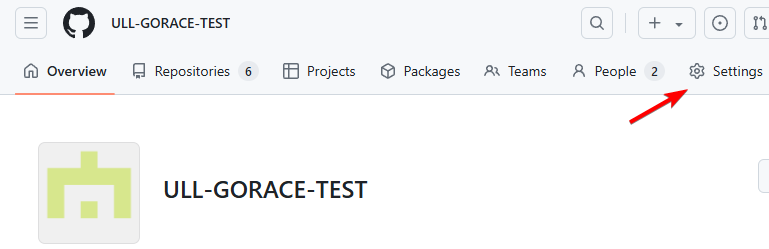
\includegraphics[width=0.5\linewidth]{images/goto-settings.png}
    \caption{Perfil de una organización en GitHub con el botón que dirige a los ajustes resaltado.}
\end{figure}

Una vez en los ajustes, localice la barra lateral izquierda y descienda hasta su final. Ahí encontrará un desplegable con los ajustes de desarrollo. Tras abrirlo, debe pinchar en la opción de GitHub Apps.

\begin{figure}[H]
    \centering
    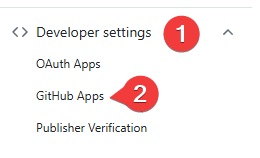
\includegraphics[width=0.5\linewidth]{images/dev-setting-gapps.png}
    \caption{Barra lateral de los ajustes de la organización mostrando la opción para ir a las GitHub Apps.}
\end{figure}

En la página en la que nos encontramos, pulsaremos el botón que dice ``New GitHub App''.

\begin{figure}[H]
    \centering
    
\includegraphics[width=0.5\linewidth]{images/new-app-btn.png}
    \caption{Botón para crear una nueva GitHub App.}
\end{figure}

En el formulario que se nos presenta, introduciremos un nombre que nos parezca adecuado y haremos lo mismo para la dirección de nuestra \textit{homepage}. En ''Callback URL'' introduciremos ''{\tt http://127.0.0.1/callback}'', desmarcaremos las opciones de ''{\tt Expire user authorization tokens}'' y ``{\tt Request user authorization (OAuth) during installation}'' si están seleccionadas, y marcaremos la opción de '{\tt 'Enable Device Flow}''.

En el apartado de \textit{webhook} estableceremos la URL a la dirección de la máquina que va a servir GH2GR Server, añadiéndole el protocolo \acrshort{HTTP} o \acrshort{HTTPS} según corresponda y añadiendo ``{\tt /hook}'' como sufijo. Así pues, si el dominio es ''{\tt gh2gr.my-domain.example}'' y sirve el contenido por medio de \acrshort{HTTP}, introduciríamos la dirección ``{\tt http://gh2gr.my-domain.example/hook}''. 

También en el apartado de \textit{webhook} especificaremos un secreto, que será un texto aleatorio y seguro que debemos recordar para más adelante.

En el apartado de permisos, dentro de los permisos de repositorio, dotaremos a la aplicación de acceso de lectura a ''Actions'', ''Checks'' y ``Metadata''. Luego, más abajo, indicaremos que nos queremos suscribir al evento de ''Workflow job''.

Concluiremos decidiendo si queremos que nuestra aplicación solo pueda ser instalada en nuestra organización o si puede ser instalada en cualquiera. Esta decisión es libre, pero se debe tener en cuenta que la aplicación debe estar instalada en todas las organizaciones donde se quiera usar GH2GR. Una vez elegido, pulsaremos el botón de ''{\tt Create GitHub App}''.

\begin{figure}
    \centering
    \begin{subfigure}{0.24\textwidth}
        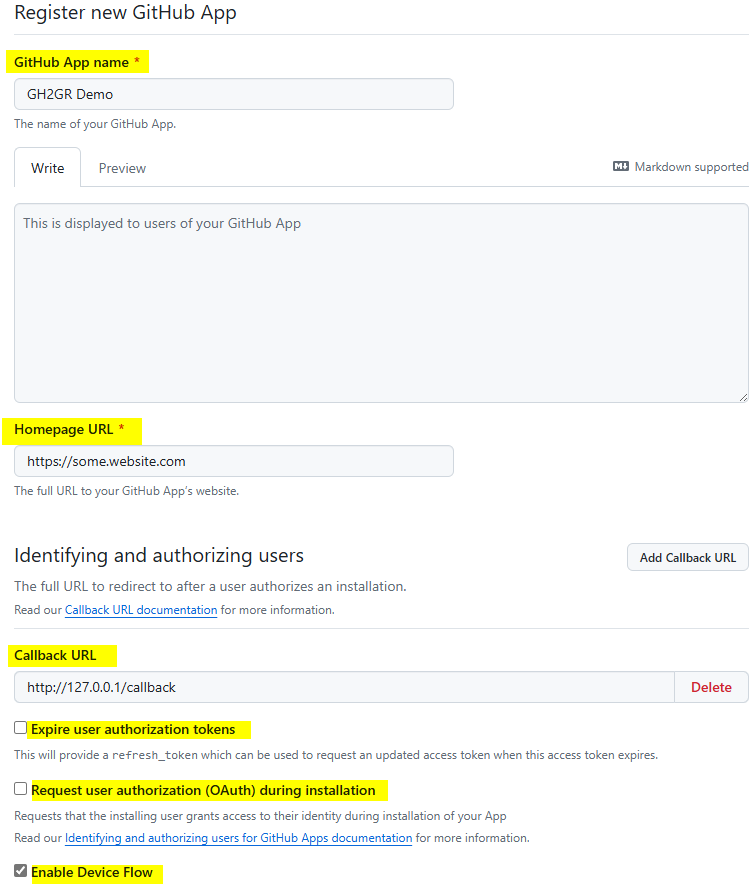
\includegraphics[width=\linewidth]{images/create-app-form-1.png}
    \end{subfigure}
    \hspace*{\fill}   % maximize separation between the subfigures
    \begin{subfigure}{0.24\textwidth}
        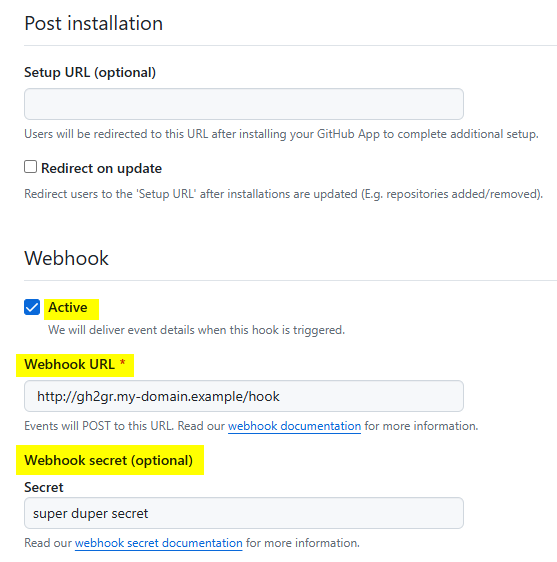
\includegraphics[width=\linewidth]{images/create-app-form-2.png}
    \end{subfigure}
    \hspace*{\fill}   % maximize separation between the subfigures
    \begin{subfigure}{0.24\textwidth}
        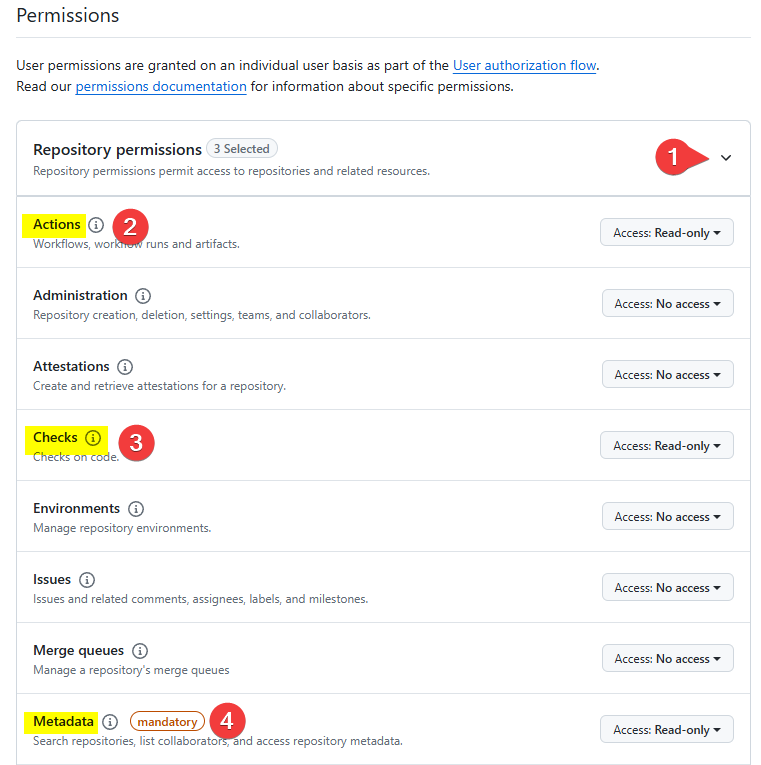
\includegraphics[width=\linewidth]{images/create-app-form-3.png}
    \end{subfigure}
    \hspace*{\fill}   % maximize separation between the subfigures
    \begin{subfigure}{0.24\textwidth}
        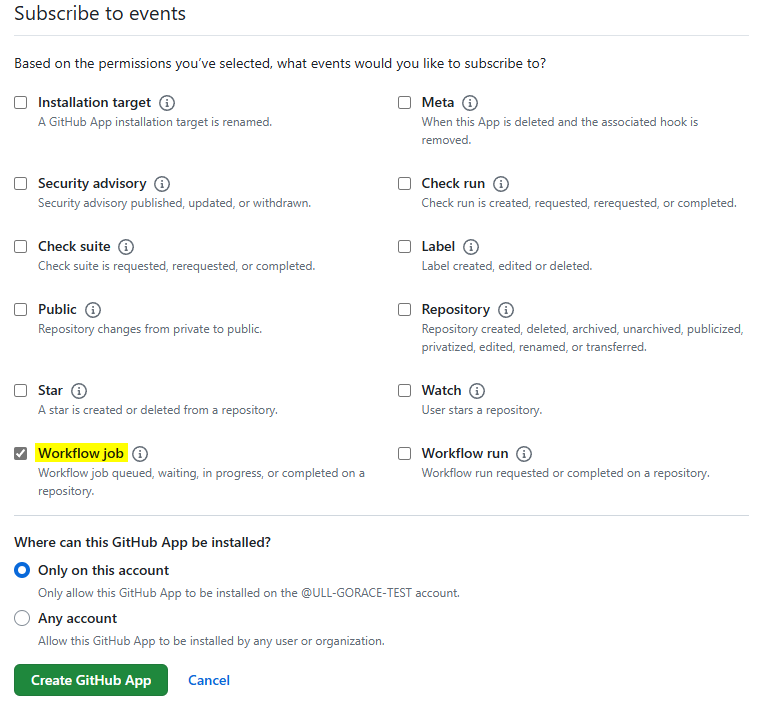
\includegraphics[width=\linewidth]{images/create-app-form-4.png}
    \end{subfigure}
    \caption{Formulario para la creación de la GitHub App con los campos ha cambiar resaltados en amarillo.}
\end{figure}

Si todo sale bien, ya se habrá creado nuestra GitHub App. Pero nuestro trabajo todavía no ha acabado, pues necesitamos generar la clave secreta que permitirá a GH2GR Server actuar como nuestra GitHub App. Para generar dicha clave, descenderemos en la página que nos ha llevado GitHub hasta llegar al apartado de ''Private Keys''. Cuando lleguemos a él, pulsaremos el botón verde que dice ''Generate a private key''. En cuanto lo pulsemos, se generará una clave y el navegador intentará descargarla, tal como se puede apreciar en la figura \ref{fig:download-secret-key}. Es importante que la guardemos en un lugar seguro, pues la necesitaremos más adelante y no puede volver a ser descargada. No obstante, si la perdemos, siempre podemos pulsar otra vez el botón de ''Generate a private key'' (que se habrá desplazado ligeramente más arriba) y, posteriormente, eliminar la clave anteriormente creada. Esto último tiene que hacerse en este orden, pues GitHub no permite eliminar la única clave privada.

Otra cosa que debemos hacer mientras estamos por esta página es apuntar el ''{\tt App ID}'' que aparece al principio de la página tal y como se puede ver en la figura \ref{fig:gh-app-id}. Necesitaremos este identificar para configurar nuestro servidor en el aparado \ref{title:config-server}.

\begin{figure}
    \centering
    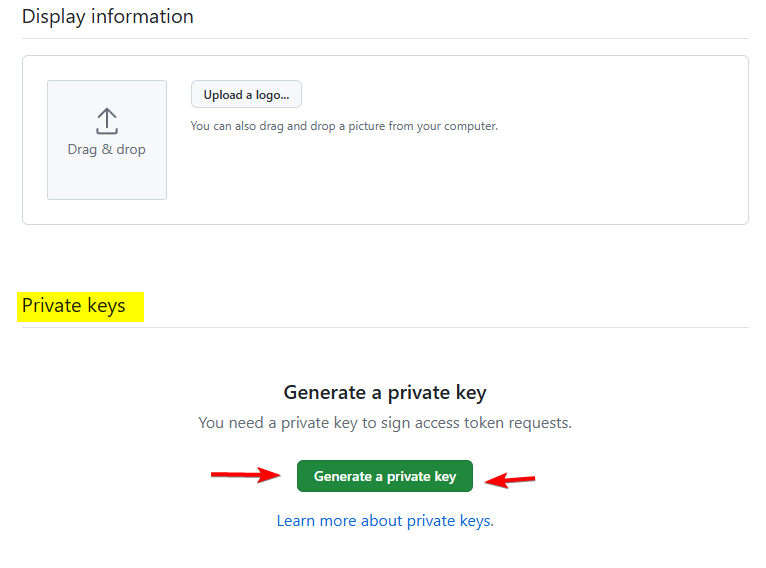
\includegraphics[width=0.5\linewidth]{images/generate-secret-key-.png}
    \caption{Botón para crear la clave privada.}
\end{figure}

\begin{figure}
    \centering
    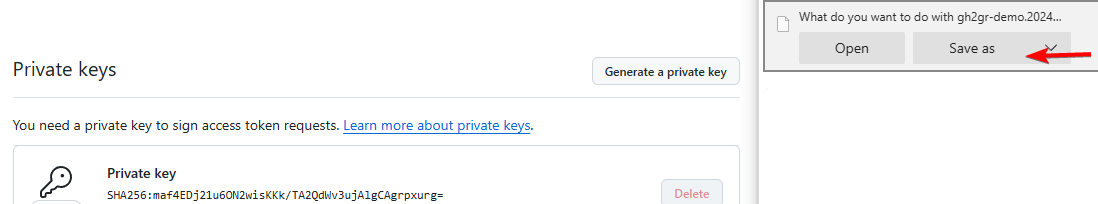
\includegraphics[width=0.5\linewidth]{images/generate-secret-key-download.png}
    \caption{Clave privada creada y el navegador ofreciendo su descarga.}
    \label{fig:download-secret-key}
\end{figure}

\begin{figure}
    \centering
    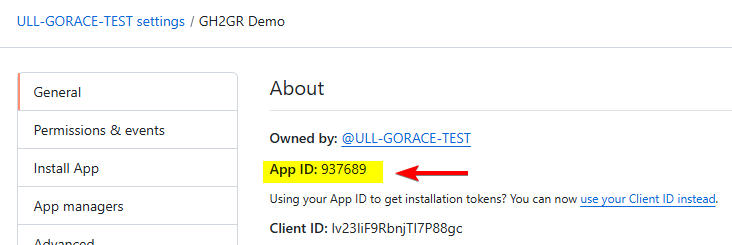
\includegraphics[width=0.75\linewidth]{images/gh-app-id.png}
    \caption{Lugar donde encontrar el App ID de nuestra GitHub App}
    \label{fig:gh-app-id}
\end{figure}

\section{Construir y distribuir el servidor}
Como ya se comentó en el apartado \ref{title:gh2gr-server-build-and-deploy}, GH2GR Server se construye utilizando contenedores \acrshort{OCI}. Por lo tanto, el único software que necesitamos tener instalado en el equipo con el que queremos construir el servidor es un motor de contenedores, específicamente uno capaz de crear imágenes \acrshort{OCI} a partir de ficheros Containerfile. En los ejemplos a continuación se usará Podman~\cite{podmanWhatPodman}. Sin embargo, esto es una preferencia personal y puede ser sustituido por cualquier otro, como Docker~\cite{dockerDockerEngine} o Containerd (nerdctl)~\cite{githubGitHubContainerdnerdctl}, por nombrar algunos ejemplos. De hacerlo, se deberán ajustar los comandos a ejecutar para satisfacer cualquier motor que se haya preferido usar. En el caso de Docker y Nerdctl, los comandos son iguales a los de Podman, por lo que solo es necesario cambiar ''podman'' por ''docker'' o ''nerdctl'', según corresponda. Si se desea usar otro motor, descubrir qué comando utilizar se deja como ejercicio al lector.

\begin{sloppypar}
Para construir la aplicación, nos dirigiremos a la raíz del repositorio de código y ejecutaremos el comando \texttt{podman build -t <usuario>/gh2gr-server -f Containerfile.server .}, sustituyendo ''<usuario>'' por nuestro propio nombre de usuario. Con la ejecución de ese comando, todas las dependencias necesarias serán descargadas, por lo que necesitaremos una conexión a internet, y se construirá una imagen \acrshort{OCI} con el binario de GH2GR Server y el entorno mínimo para poder ejecutarlo. Si todo ha salido bien, deberíamos ver una salida similar a la figura \ref{fig:build-server}.
\end{sloppypar}

\begin{figure}[H]
    \centering
    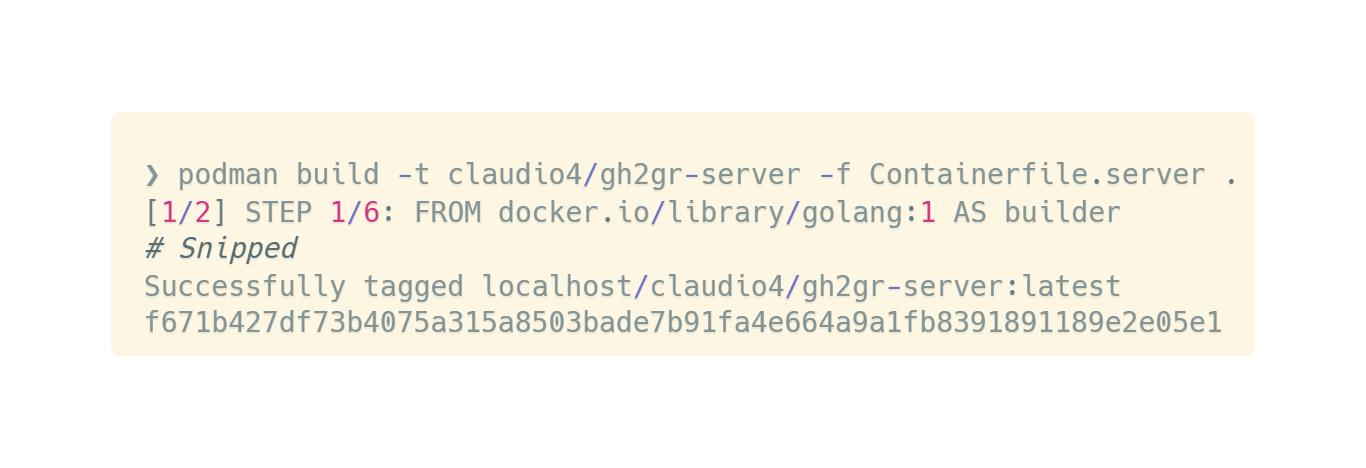
\includegraphics[width=0.75\linewidth]{images/build-server.png}
    \caption{Ejecución del comando de construcción de GH2GR Server. Parte de la salida omitida por brevedad.}
    \label{fig:build-server}
\end{figure}

Podemos asegurarnos de que todo ha funcionado correctamente tratando de ejecutar el programa. Para simplificar la prueba, solo llamaremos al subcomando de ayuda, que debe imprimirnos el texto de ayuda del programa. Esto lo haremos ejecutando \texttt{podman run --rm <usuario>/gh2gr-server help}. Con dicho comando se creará un contenedor efímero que ejecutará la ayuda de GH2GR Server y luego será eliminado. Si no se nos presenta ningún problema, deberíamos tener una salida igual a la de la figura \ref{fig:server-help}.


\begin{figure}
    \centering
    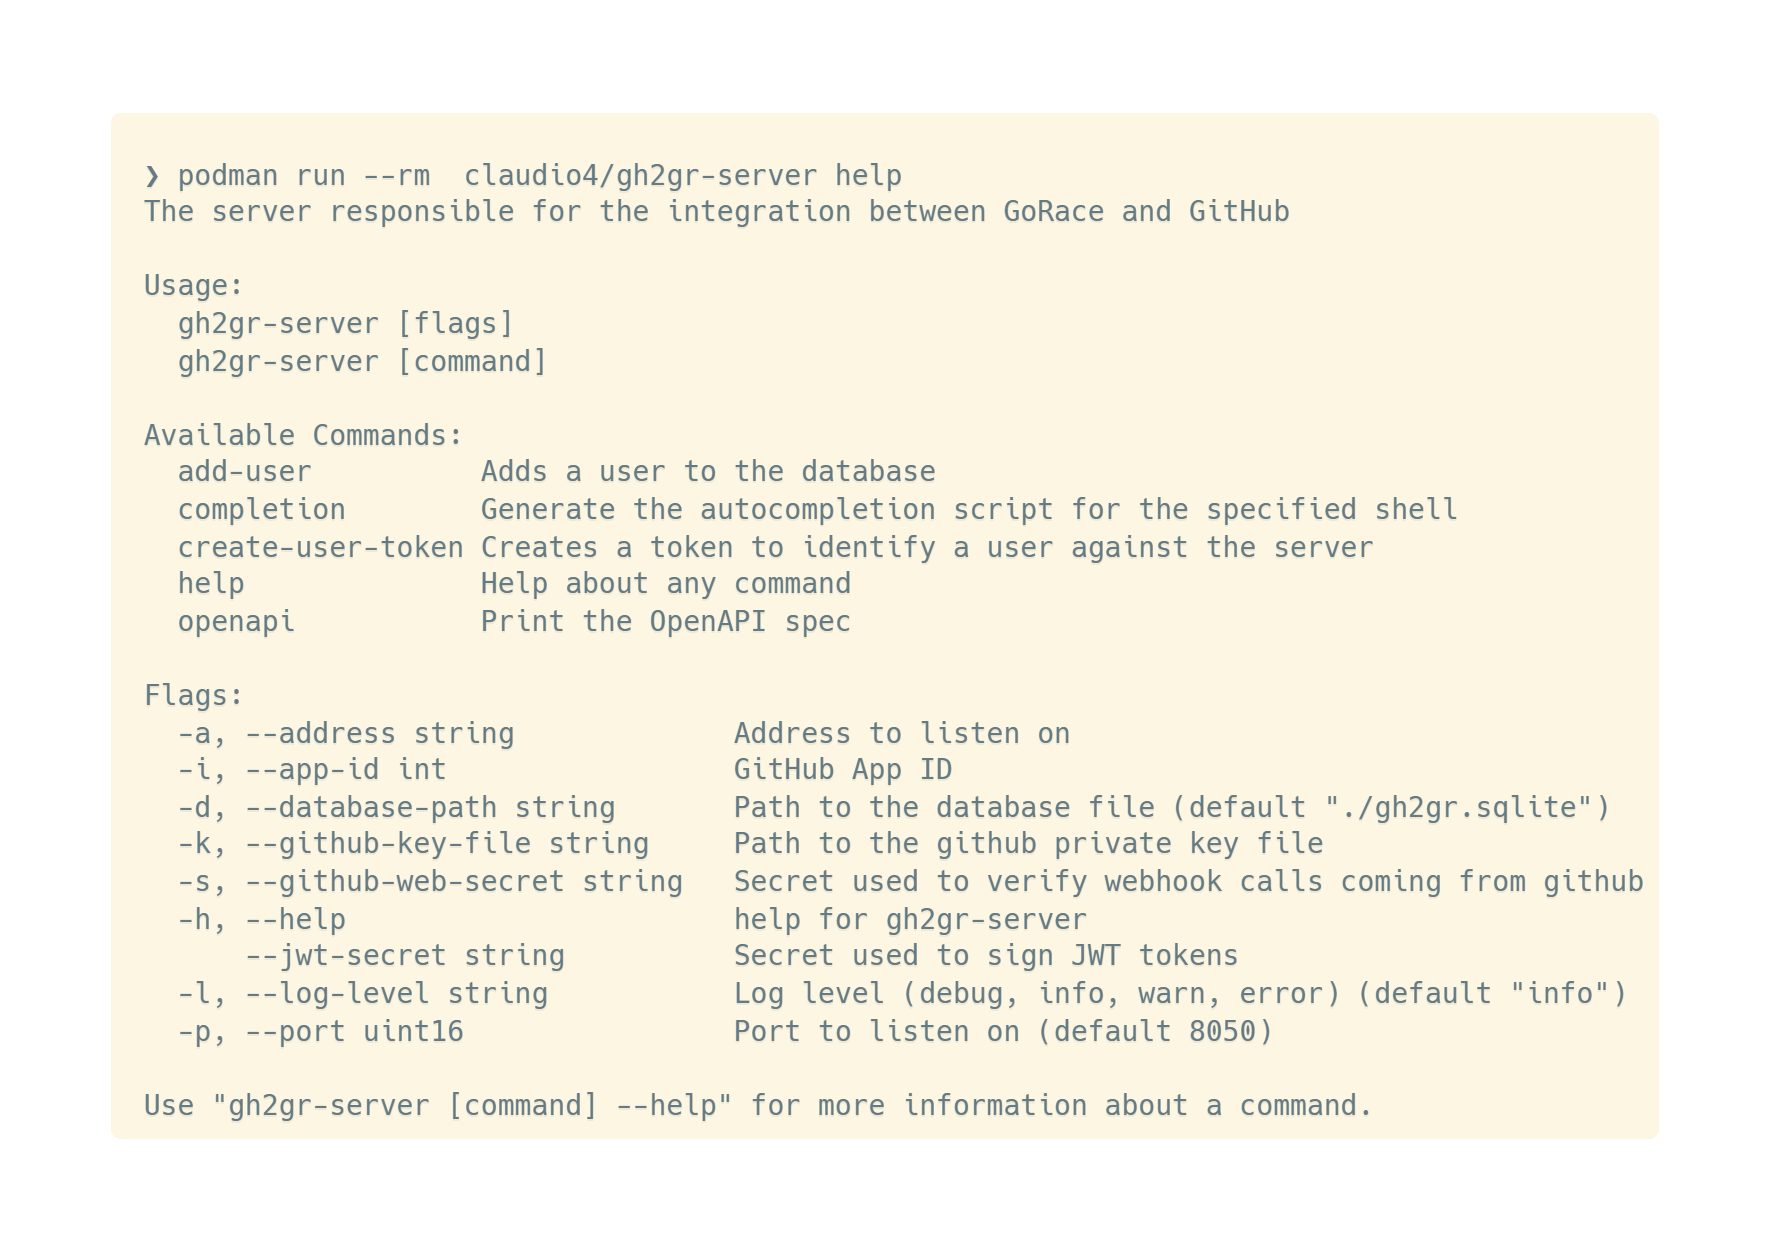
\includegraphics[width=0.75\linewidth]{images/server-help.png}
    \caption{Salida del comando de ayuda de Gh2GR Server.}
    \label{fig:server-help}
\end{figure}

Ahora que ya tenemos una imagen funcional del servidor, lo que resta es saber cómo poder transferirla a la máquina servidor que vaya a ser la encargada de servir GH2GR Server. Una opción completamente válida es simplemente construir la imagen directamente en la máquina objetivo y ahorrarse el tener que moverla, ya que no se requiere más software especializado en la máquina que el motor de contenedores que necesita para poder ejecutar la imagen \acrshort{OCI} de todas formas. Aun válida, solo contar con esta opción es restrictivo, por eso a continuación se van a enseñar dos métodos para poder distribuir la imagen.

\subsection{Distribución mediante fichero}
Es posible exportar nuestra imagen \acrshort{OCI} a un único fichero tar, el cual luego podremos transferir a donde necesitemos utilizando cualquier método de transferencia de archivos. Para lograr esto, solo tenemos que ejecutar el comando \texttt{podman image save <usuario>/gh2gr-server -o gh2gr-server.tar}. Tras ver una salida como la de la figura \ref{fig:export-oci-image}, contaremos con un archivo ''{\tt gh2gr-server.tar}'' que podemos llevar a la máquina destino.

Una vez en la máquina destino, debemos importar la imagen antes de poder usarla. Esto lo haremos con el comando \texttt{podman image load --input gh2gr-server.tar}, suponiendo que nos encontramos en la misma carpeta que el fichero tar. Tras unos segundos, ya deberíamos contar con la imagen en nuestro sistema y estará lista para ser utilizada. Si queremos asegurarnos, podemos volver a hacer la misma comprobación ejecutando el comando de ayuda que hicimos tras construir la imagen.

\begin{figure}
    \begin{subfigure}{0.49\textwidth}
        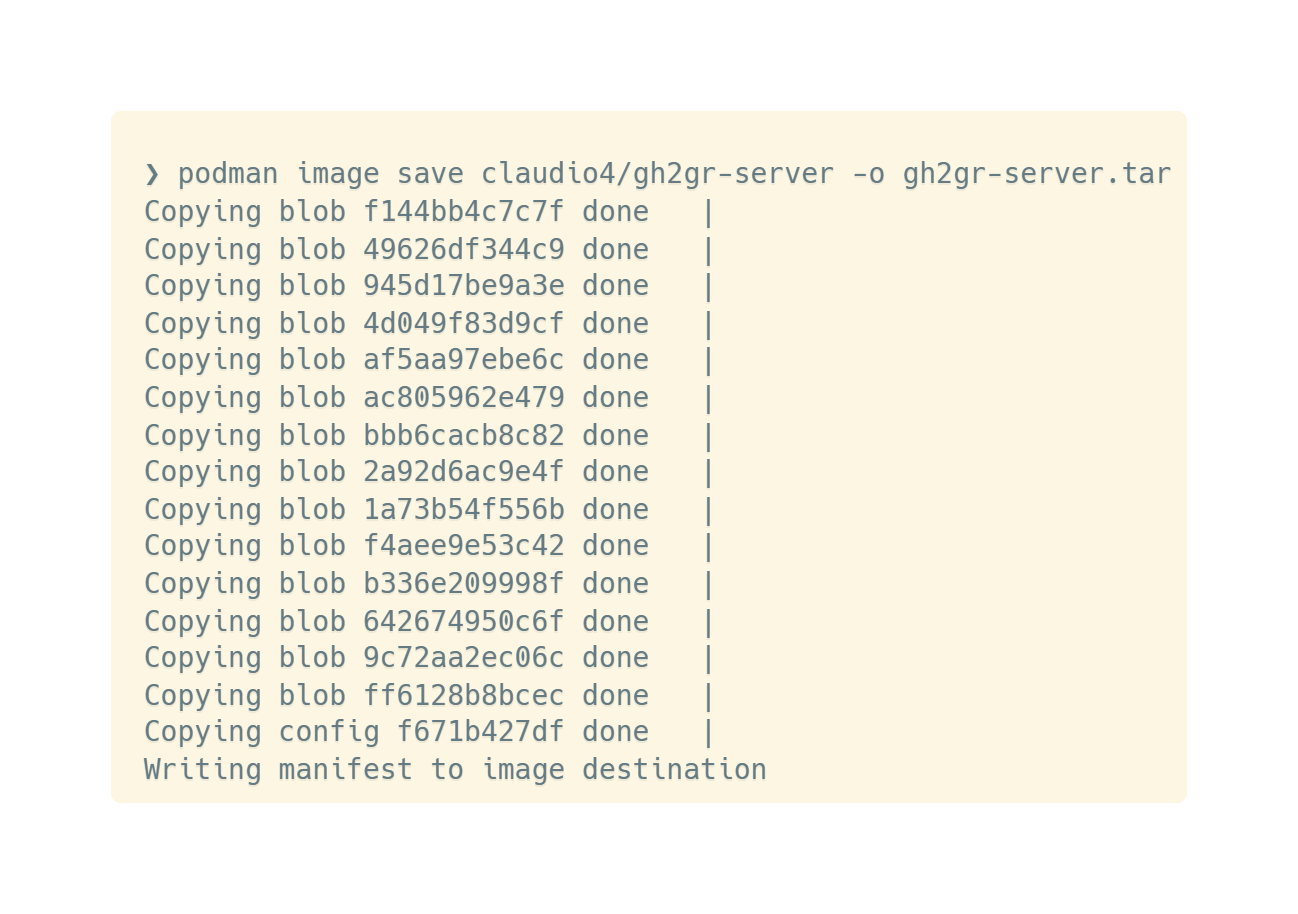
\includegraphics[width=\linewidth]{images/export-server-image.png}
        \caption{Ejecución del comando de exportado de la imagen OCI en Podman.} \label{fig:export-oci-image}
    \end{subfigure}
    \hspace*{\fill}   % maximize separation between the subfigures
    \begin{subfigure}{0.49\textwidth}
        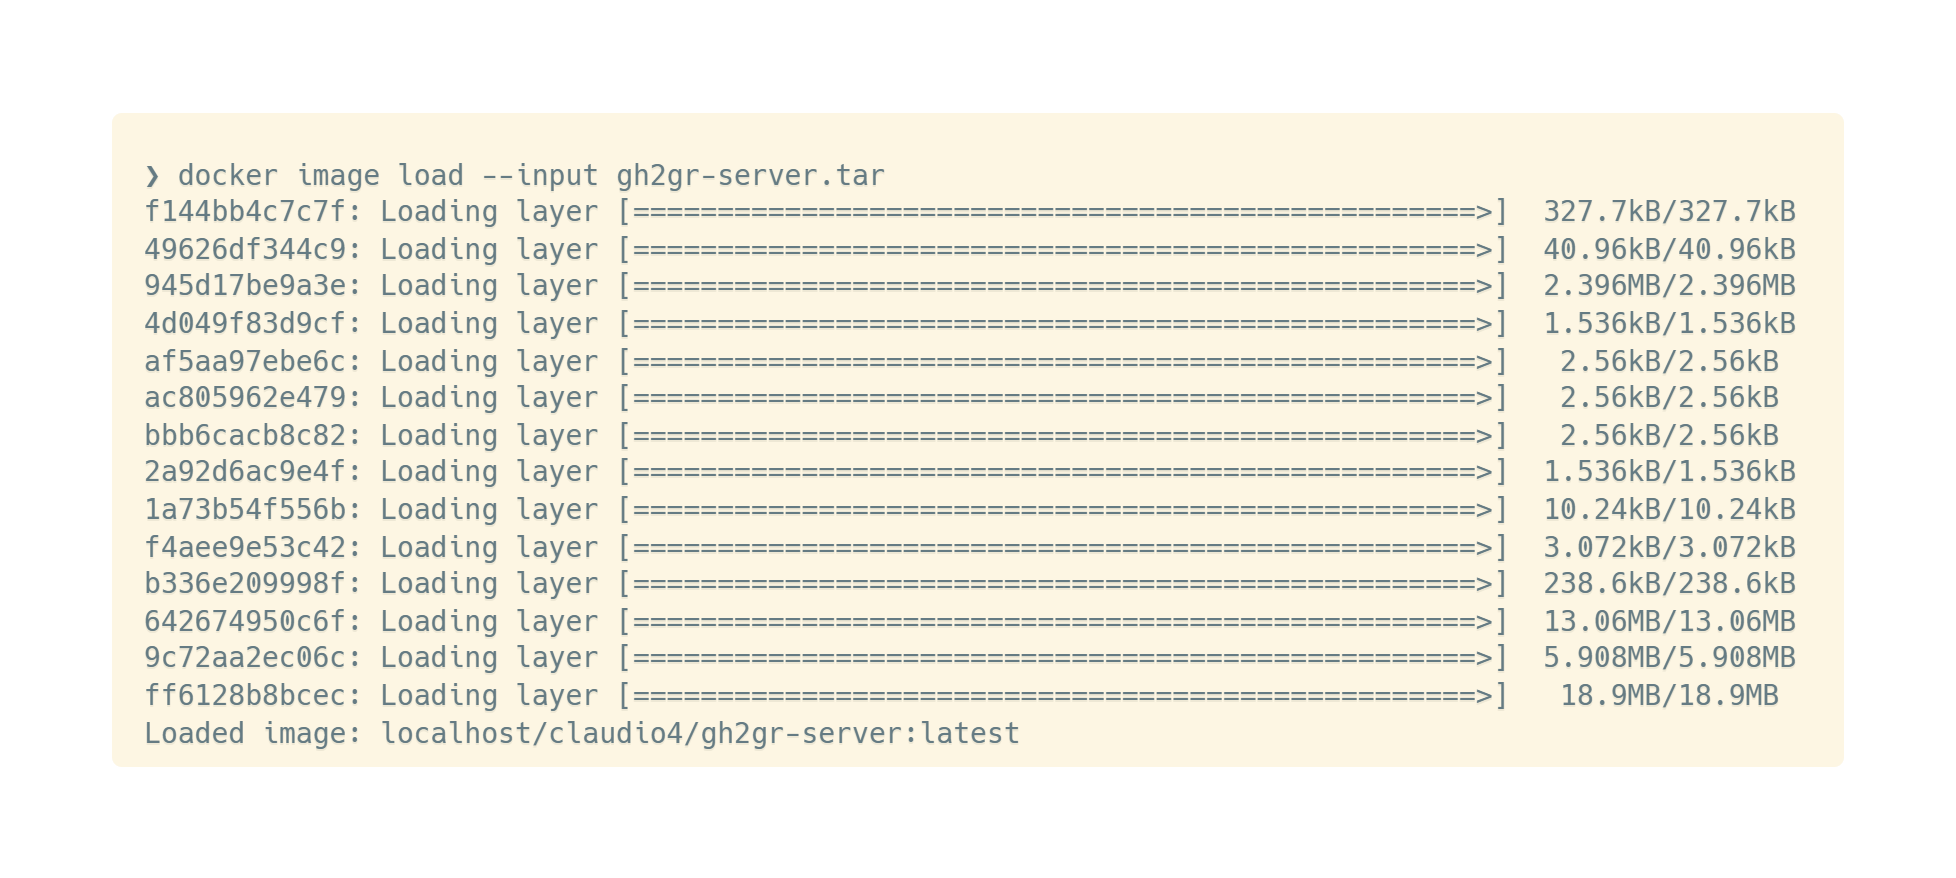
\includegraphics[width=\linewidth]{images/import-server-image.png}
        \caption{Ejecución del comando de importado de la imagen OCI. en Docker} \label{fig:import-oci-image}
    \end{subfigure}
    \caption{Importado y exportado de una imagen OCI.}
\end{figure}


\subsection{Distribución mediante un registro de imágenes OCI}
Un registro de imágenes \acrshort{OCI} es un repositorio especializado encargado de almacenar y distribuir imágenes \acrshort{OCI}~\cite{ociDistribution}. Esto lo hacen siguiendo la especificación de distribución \acrshort{OCI}. La principal ventaja que tienen es que los motores de contenedores que implementan la especificación de distribución \acrshort{OCI} son capaces de buscar en ellos y descargarse las imágenes adecuadas automáticamente.

El primer paso es escoger qué registro utilizar, ya que existen múltiples servicios en línea que podemos usar. También, por supuesto, podemos crear el nuestro propio, pero esto se sale del alcance de este documento. Para esta guía, utilizaremos Docker Hub, pero una vez más, el lector puede escoger cualquiera que le satisfaga más.

Para subir una imagen a Docker Hub, primero tendremos que registrarnos. Una vez registrado, iremos a la página principal y pincharemos en el botón de ''Create repository'' (fig. \ref{fig:docker-hub-create}). Tras pulsarlo, nos preguntará por el nombre del repositorio y por su visibilidad. Lo llamaremos ''gh2gr-server'' y procederemos a crearlo con la visibilidad que más nos convenza. Una vez creado, podemos volver a la terminal.

\begin{figure}
    \centering
    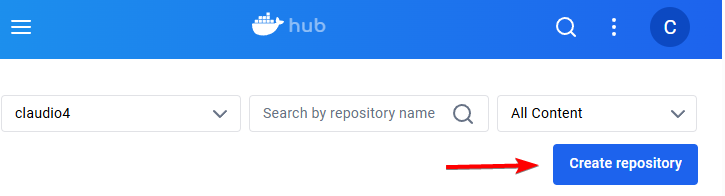
\includegraphics[width=0.75\linewidth]{images/docker-hub-create.png}
    \caption{Botón para crear un repositorio en Docker Hub}
    \label{fig:docker-hub-create}
\end{figure}

\begin{figure}
    \centering
    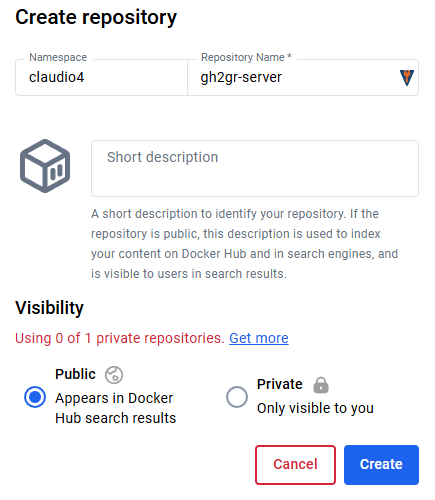
\includegraphics[width=0.75\linewidth]{images/ducker-hub-form.png}
    \caption{Formulario de creación }
\end{figure}

\begin{sloppypar}
Lo primero que tendremos que hacer en la línea de comando es iniciar sesión en Docker Hub desde Podman, si no lo hemos hecho ya. Para ello, basta con ejecutar \texttt{podman login docker.io} e introducir nuestras credenciales cuando nos las pregunte (Fig. \ref{fig:podman-login}). Ahora pasaremos a reetiquetar nuestra imagen para que esté prefijada con el dominio ''docker.io'', señalando así el repositorio en donde debe ser buscada. Para ello, ejecutamos \texttt{podman tag <usuario>/gh2gr-server docker.io/<usuario>/gh2gr-server:latest}. Es normal que este último comando no produzca salida, de hecho, esto indica que la operación se ha realizado con éxito.

\end{sloppypar}

\begin{figure}
    \centering
    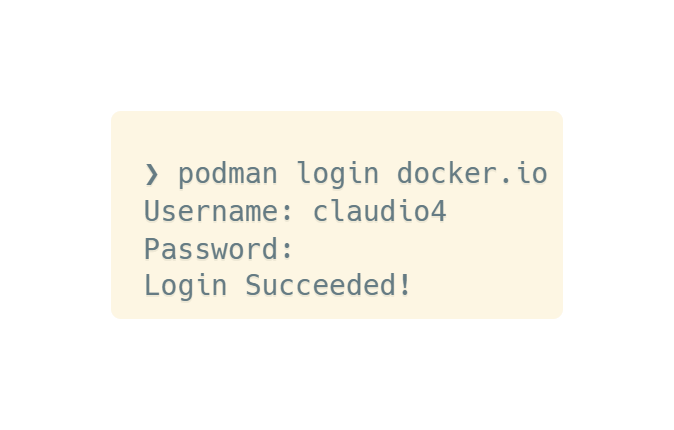
\includegraphics[width=0.75\linewidth]{images/podman-login.png}
    \caption{Iniciar sesión en Docker Hub meideante Podman.}
    \label{fig:podman-login}
\end{figure}

Ya estamos listos para subir la imagen al registro, hito que lograremos ejecutando \texttt{podman push docker.io/<usuario>/gh2gr-server:latest}. Si vemos algo similar a la figura \ref{fig:push-server-image}, significará que todo ha ido de forma correcta y nuestra imagen ya se encuentra en el registro.

\begin{figure}
    \centering
    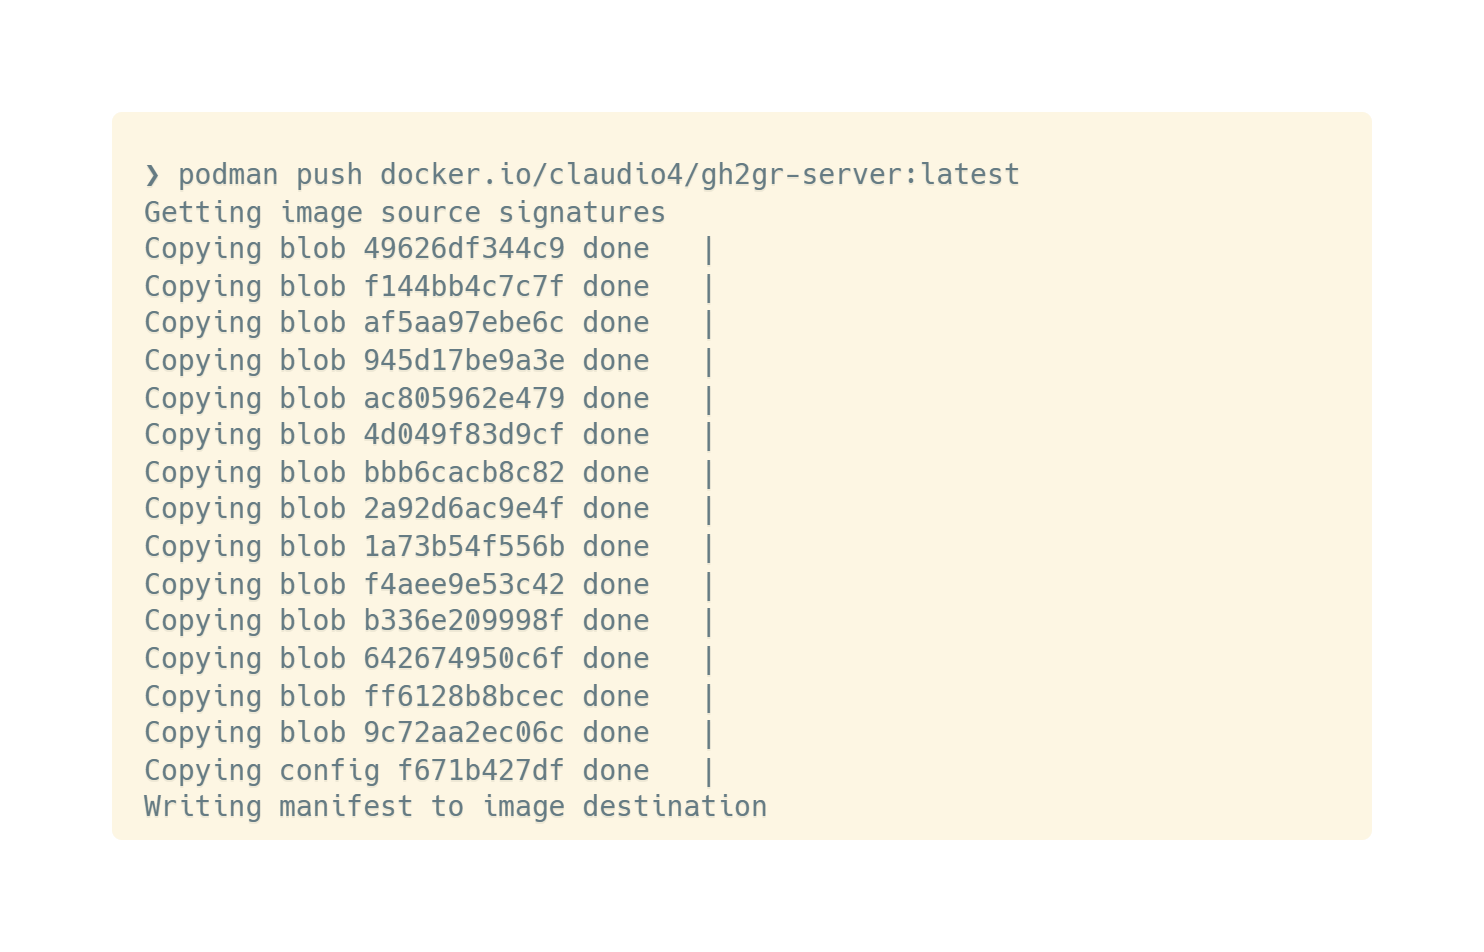
\includegraphics[width=0.75\linewidth]{images/push-server-image.png}
    \caption{Salida del comando para subir la imagen a Docker Hub}
    \label{fig:push-server-image}
\end{figure}

\begin{sloppypar}
Ahora podemos dirigirnos a nuestra máquina objetivo y simplemente tratar de utilizar la imagen como si ya estuviera ahí, pues el motor de contenedores se encargará de obtenerla por nosotros. Por tanto, si ejecutamos \texttt{podman  run  --rm docker.io/<usuario>/gh2gr-server help}, se descargará la imagen y aparecerá el texto de ayuda tal y como muestra la figura \ref{fig:server-help-remote}.
\end{sloppypar}

\begin{figure}
    \centering
    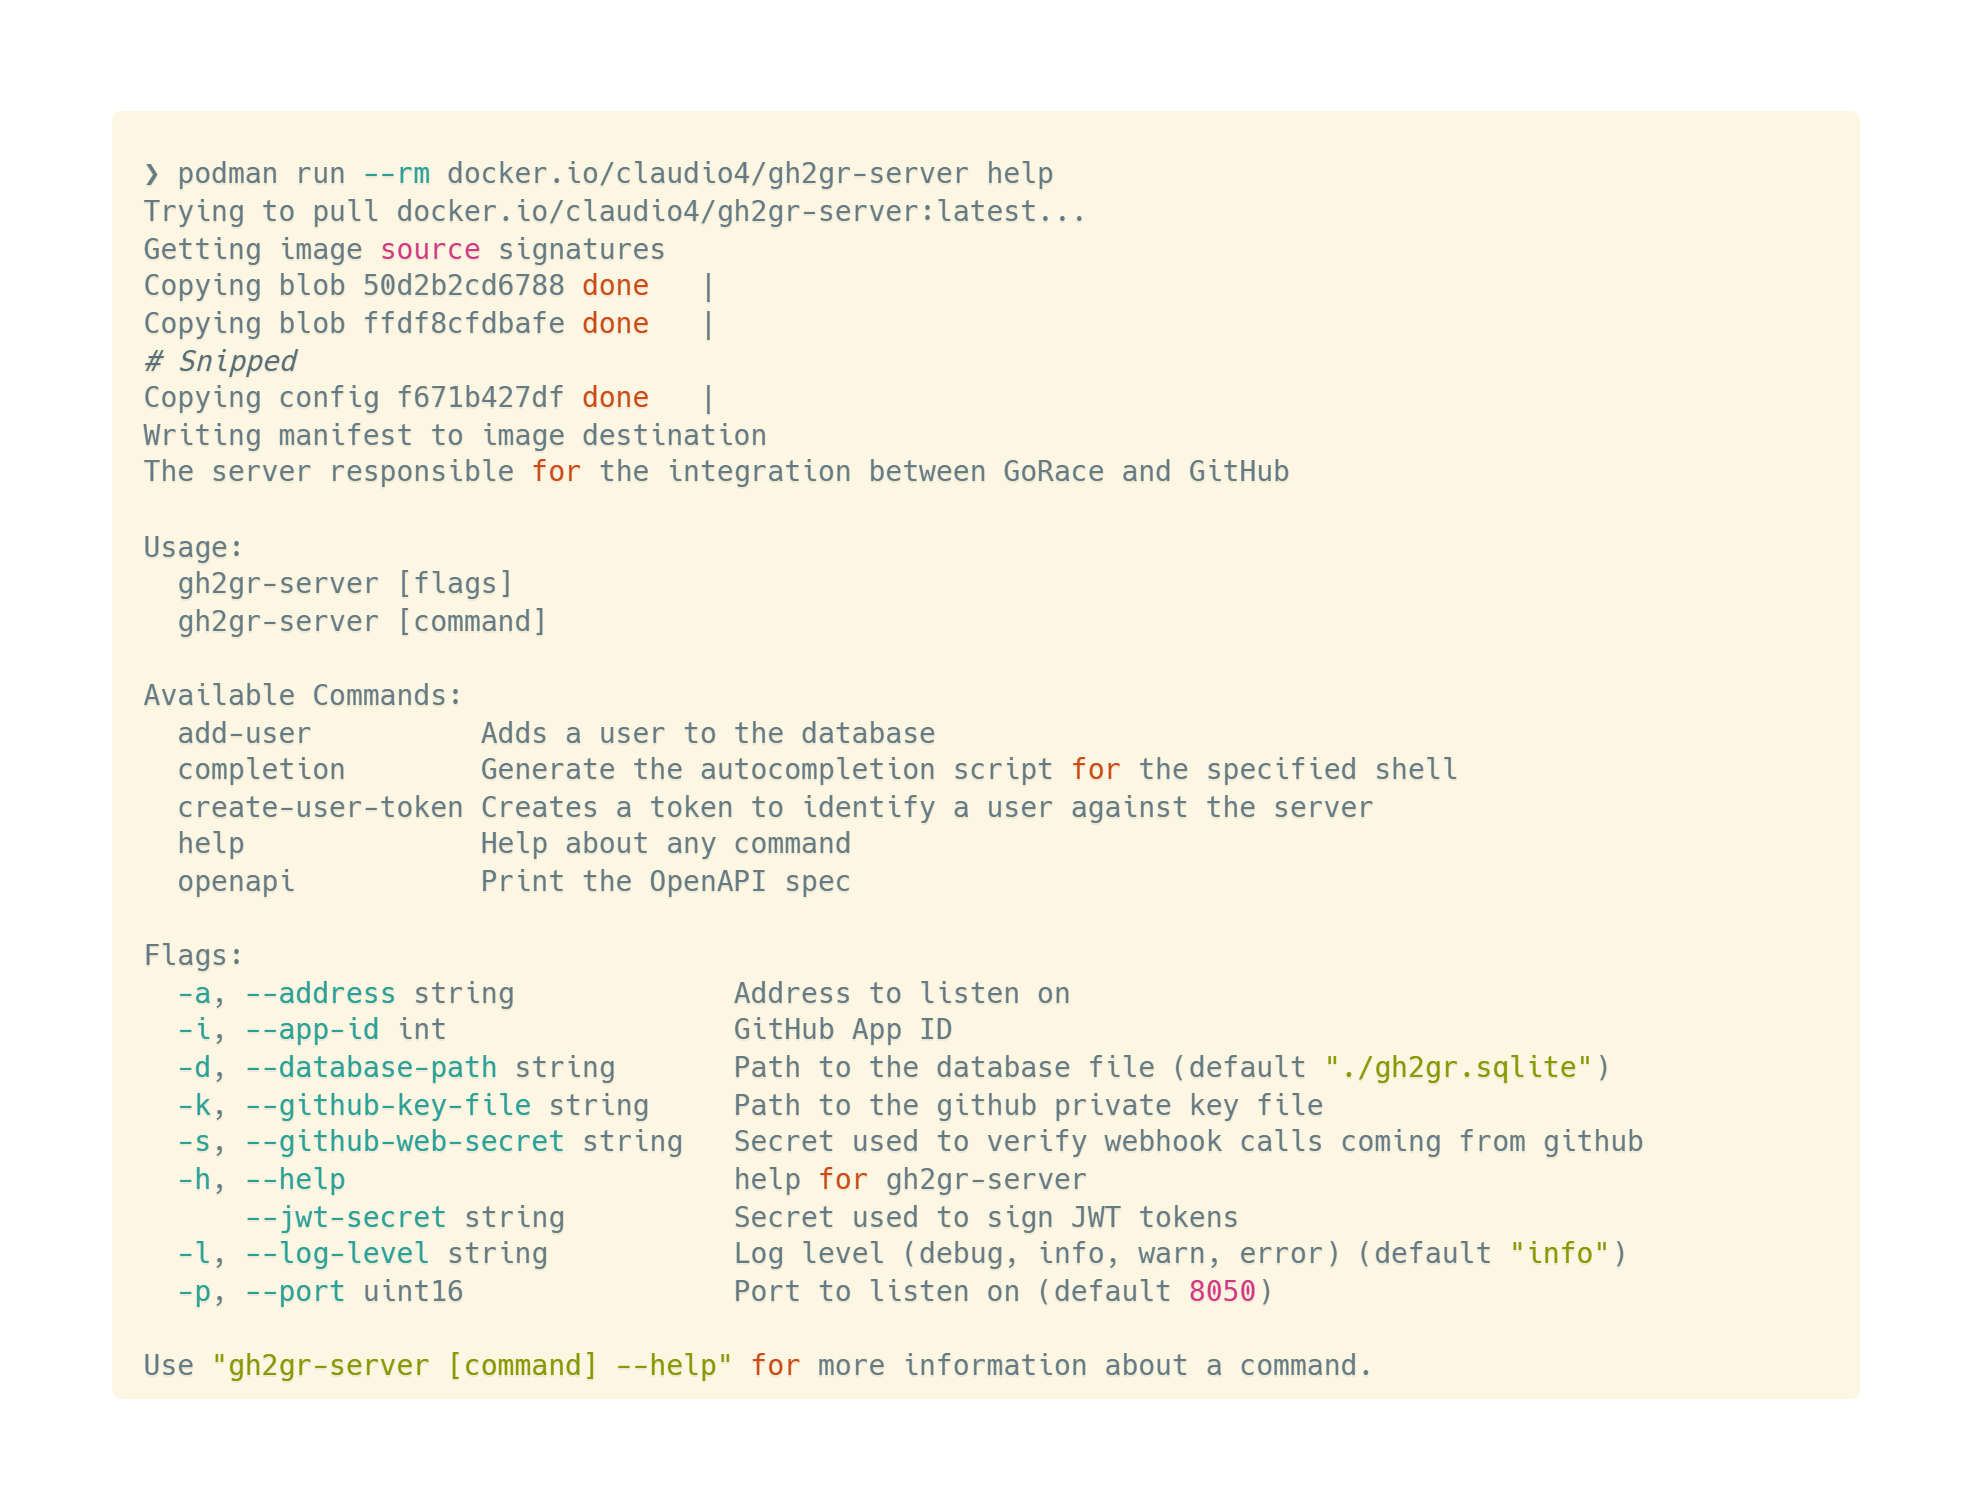
\includegraphics[width=0.75\linewidth]{images/server-help-remote.png}
    \caption{Descarga de la imagen OCI y posterior salida del comando de ayuda de Gh2GR Server.}
    \label{fig:server-help-remote}
\end{figure}

\section{Configurar el servidor} \label{title:config-server}
Ahora que ya tenemos la imagen de GH2GR Server en nuestro servidor, ha llegado la hora de configurarlo para que comience a trabajar correctamente. Lo primero que tendremos que hacer es crear una carpeta para albergar los ficheros de GH2GR Server en el lugar que nos resulte más conveniente. Una vez creada, colocaremos en ella la clave privada que obtuvimos en el apartado \ref{title:create-gh-app}.

GH2GR Server requiere que le configuremos, al menos, la GitHub App ID (obtenida al final del apartado \ref{title:create-gh-app}), la ruta de la clave secreta, el secreto para el \textit{webhook}, que también configuramos en el apartado \ref{title:create-gh-app}, y un secreto aleatorio para firmar nuestros \acrshort{JWT}. Podemos proporcionar estos detalles como parámetros, tal y como podemos ver en la figura \ref{fig:server-help}, o podemos usar variables de entorno. En caso de usar estas últimas, el nombre de cada variable será igual al del parámetro (en su versión no acortada) en mayúsculas, sustituyendo los guiones por barras bajas (\texttt{\_}) y precediéndolo de \texttt{GH2GR\_}. Así pues, si quisiéramos configurar el App ID, usaremos la variable \texttt{GH2GR\_APP\_ID}. También es importante comentar que se pueden usar a la vez parámetros y variables de entorno para configurar los distintos ajustes. Si una misma opción se configurara por ambos métodos, prevalecería el valor escogido mediante parámetros.

\begin{sloppypar}
Para lanzar nuestro contenedor correctamente configurado, usaríamos el comando de la figura \ref{fig:run-server}. Si hemos hecho todo correctamente, deberíamos ver un mensaje indicándonos que el servidor \acrshort{HTTP} se ha iniciado en el puerto 8050.
\end{sloppypar}


\begin{figure}[H]
\begin{minted}[tabsize=2,breaklines,fontsize=\footnotesize]{bash}
podman run -p 8050:8050 -v "/path/to/gh2gr-folder:/data" \
-e GH2GR_APP_ID=937689 \
-e GH2GR_GITHUB_KEY_FILE=/data/key.pem \
-e GH2GR_GITHUB_WEB_SECRET=webhoo-secret \
-e GH2GR_JWT_SECRET=very-random-secret \
-e GH2GR_DATABASE_PATH=/data/gh2gr.sqlite \
<usuario>/gh2gr-server
\end{minted}
\caption{Comando para ejecutar GH2GR Server}
\label{fig:run-server}
\end{figure}

Desglosemos rápidamente el comando:
\begin{itemize}
    \item \textbf{podman run}: Lanzamos un contenedor con Podman.
    \item \textbf{-p 80:8050}: Enlazamos el puerto 80 de nuestra máquina con el puerto 8050 del contenedor.
    \item \textbf{-v "/path/to/gh2gr-folder:/data"}: Montamos la carpeta que creamos al inicio en la ruta /app dentro del contenedor.
    \item \textbf{-e GH2GR\_APP\_ID=937689}: Establecemos el GitHub App ID con una variable de entorno.
    \item \textbf{-e GH2GR\_GITHUB\_KEY\_FILE=/data/key.pem}: Indicamos la ruta a nuestra clave privada mediante una variable de entorno. Como la ruta es relativa al interior del contenedor, usamos el /data que montamos antes.
    \item \textbf{-e GH2GR\_GITHUB\_WEB\_SECRET=webhook-secret}: Configuramos el secreto del \textit{webhook} con una variable de entorno.
    \item \textbf{-e GH2GR\_JWT\_SECRET=very-random-secret}: Configuramos el secreto de nuestros \acrshort{JWT} con una variable de entorno.
    \item \textbf{-e GH2GR\_DATABASE\_PATH=/data/gh2gr.sqlite}: Indicamos dónde se debe guardar la base de datos mediante una variable de entorno. La ruta tiene que ubicarse dentro de /data; de lo contrario, la base de datos no persistirá si el contenedor es borrado.
    \item \textbf{<usuario>/gh2gr-server}: La imagen que debe ejecutar Podman, en concreto, la que creamos nosotros.
\end{itemize}

Llegados a este punto, ya tenemos nuestro servidor prácticamente listo. Lo único que nos queda es buscar un método para persistir la ejecución del comando y asegurarnos de que el puerto 80 esté expuesto a través de internet. Dado que el cómo conseguir esto depende mucho del entorno en el que se ha decidido ejecutar el contenedor, se ha dejado el resolver estas cuestiones como un ejercicio para el lector.


\section{Añadir usuarios y crear credenciales} \label{title:add-user}
Ahora vamos a proceder a añadir usuarios docentes para que puedan usar GH2GR Server. Esta acción la haremos desde la línea de comandos de la máquina que sirve GH2GR Server.
\begin{sloppypar}
El único detalle que necesitaremos conocer de ellos es el nombre de usuario. Una vez nos hemos decidido por uno, podemos agregarlo ejecutando 

\texttt{podman run --rm -v "/path/to/gh2gr-folder:/data -e GH2GR\_DATABASE\_PATH=/data/gh2gr.sqlite <usuario>/gh2gr-server add-user prueba1}

El comando nos responderá con el ID del usuario, como se puede ver en la figura \ref{fig:add-user}.
\end{sloppypar}

\begin{figure}
    \centering
    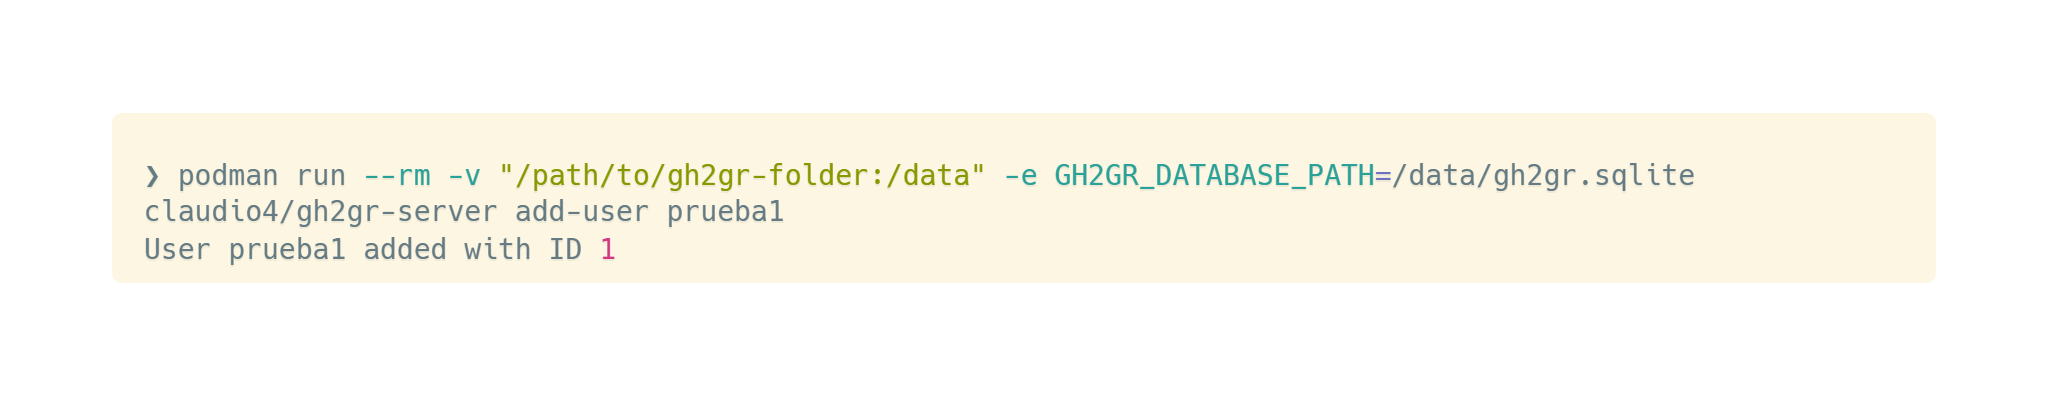
\includegraphics[width=0.75\linewidth]{images/add-user.png}
    \caption{Salida del comando que agrega un usuario a GH2GR Server.}
    \label{fig:add-user}
\end{figure}

\begin{sloppypar}
Ahora que hemos añadido al usuario, sería conveniente generarle unas credenciales para que pueda iniciar sesión. Esto lo podemos hacer con el comando 

\texttt{podman run --rm -v "/path/to/gh2gr-folder:/data -e GH2GR\_JWT\_SECRET=very-random-secret -e GH2GR\_DATABASE\_PATH=/data/gh2gr.sqlite <usuario>/gh2gr-server create-user-token prueba1}

El comando nos devolverá inmediatamente el token que el usuario necesita para iniciar sesión desde GH2GR Client, tal y como se puede ver en la figura \ref{fig:create-user-token}.
\end{sloppypar}

\begin{figure}
    \centering
    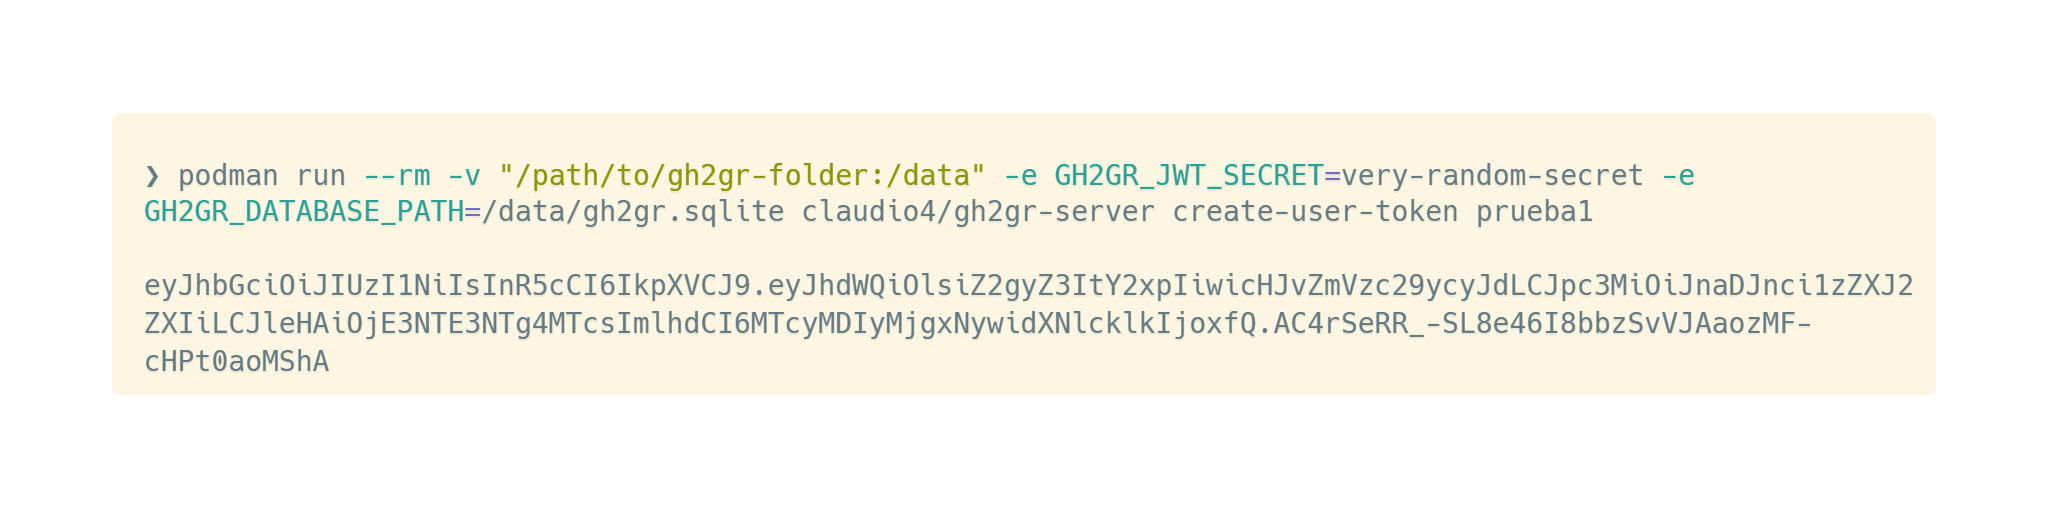
\includegraphics[width=0.75\linewidth]{images/create-user-token.png}
    \caption{Salida del comando para crear las credenciales de un usuario de GH2GR Server.}
    \label{fig:create-user-token}
\end{figure}

\section{Construcción del cliente}
El cliente es una aplicación más sencilla que el servidor y no requiere de CGO, así que nos aventuraremos a compilarla directamente sin usar contenedores. Esto significa que necesitamos tener instalado el SDK de Go en nuestra máquina. Las instrucciones varían según el sistema operativo, pero son sencillas y están disponibles en la página oficial del proyecto~\cite{installGo}.

Si ya tenemos el SDK instalado, podemos construir la aplicación simplemente yendo a la raíz del repositorio y ejecutando \texttt{go build -o gh2gr cmd/gh2gr-cli/main.go}. Go se encargará de descargar las dependencias externas (cosa que solo hace la primera vez, pero requiere conexión a internet) y compilará nuestro binario con el nombre ``gh2gr''. Podemos probar que funciona correctamente ejecutándolo con \texttt{./gh2gr}. Nos debería devolver una pantalla como la de la Figura \ref{fig:client-root-help}.

\begin{figure}
    \centering
    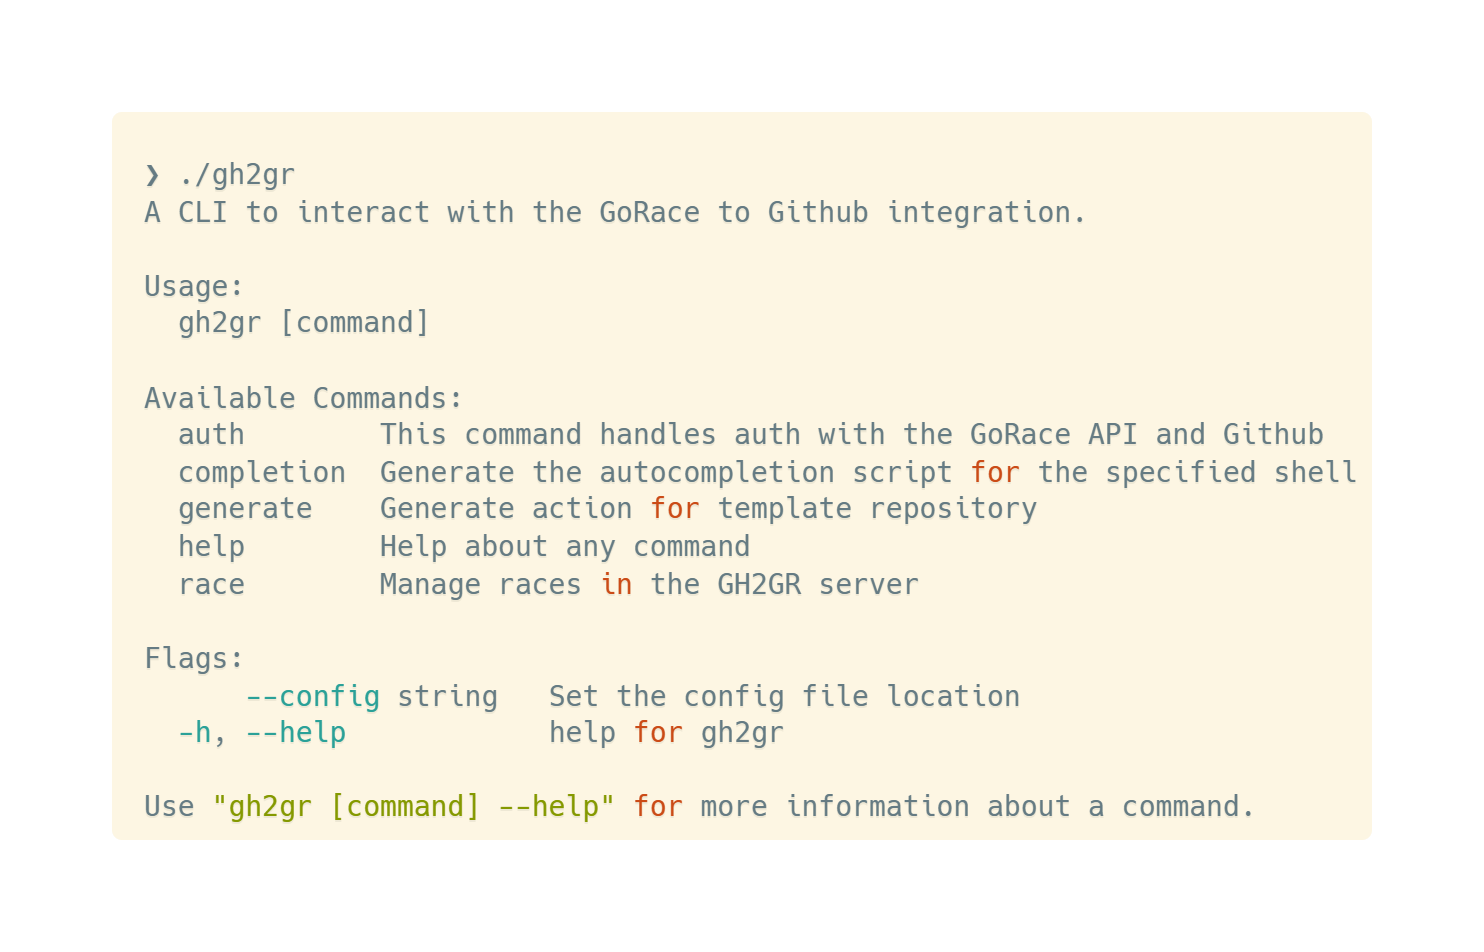
\includegraphics[width=0.75\linewidth]{images/client-root-help.png}
    \caption{Salida del comando principal de GH2GR Client.}
    \label{fig:client-root-help}
\end{figure}

\section{Configurar el cliente}
Ahora que ya tenemos el servidor funcionando y el cliente compilado, lo que nos resta es configurar el cliente, y eso realmente se traduce en iniciar sesión con él tanto en GitHub como en GH2GR Server.

Para iniciar sesión en GitHub, ejecutaremos el comando \texttt{gh2gr auth github login}. El comando nos dará un código y nos pedirá que pulsemos \textit{Enter} para continuar al navegador (Figura \ref{fig:gh-client-login:cli}). Al pulsarlo, se nos llevará a una página de GitHub donde tendremos que iniciar sesión, si no lo hemos hecho ya, e introducir el código que nos proporcionó GH2GR Client al ejecutarlo (Figura \ref{fig:gh-client-login:code}). Tras introducirlo, nos pedirá que confirmemos si efectivamente queremos permitir a GH2GR Client acceder a nuestra cuenta (Figura \ref{fig:gh-client-login:authz}). Responderemos que sí. Después, veremos que GH2GR Client nos imprime nuestro código de acceso y sale. No es necesario que guardemos este token, ya que la propia aplicación lo ha guardado en su configuración.

\begin{figure}
    \begin{subfigure}{0.32\textwidth}
        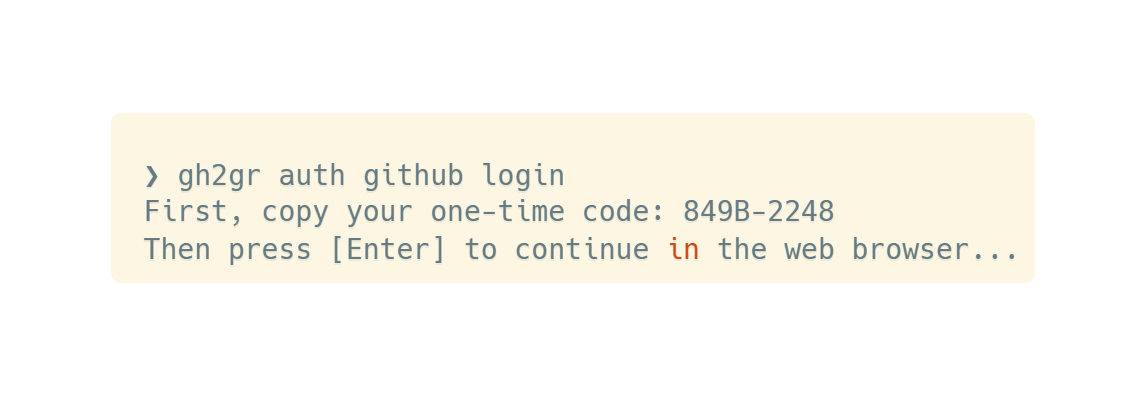
\includegraphics[width=\linewidth]{images/client-gh-login-code.png}
        \caption{Salida inicial del comando para iniciar sesión en GitHub desde GH2GR Client.}
        \label{fig:gh-client-login:cli}
    \end{subfigure}
    \hspace*{\fill}
    \begin{subfigure}{0.32\textwidth}
        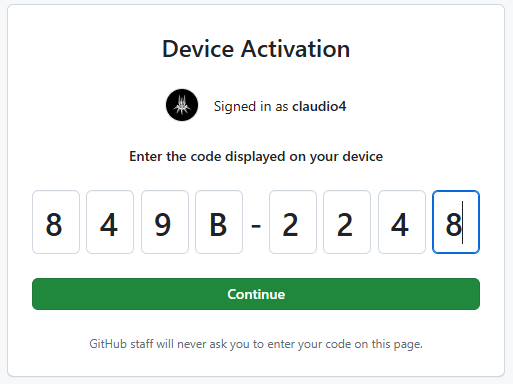
\includegraphics[width=\linewidth]{images/insert-gh-auth-code.png}
        \caption{Pantalla donde debemos introducir el código para iniciar sesión.}
        \label{fig:gh-client-login:code}
    \end{subfigure}
    \hspace*{\fill}
    \begin{subfigure}{0.32\textwidth}
        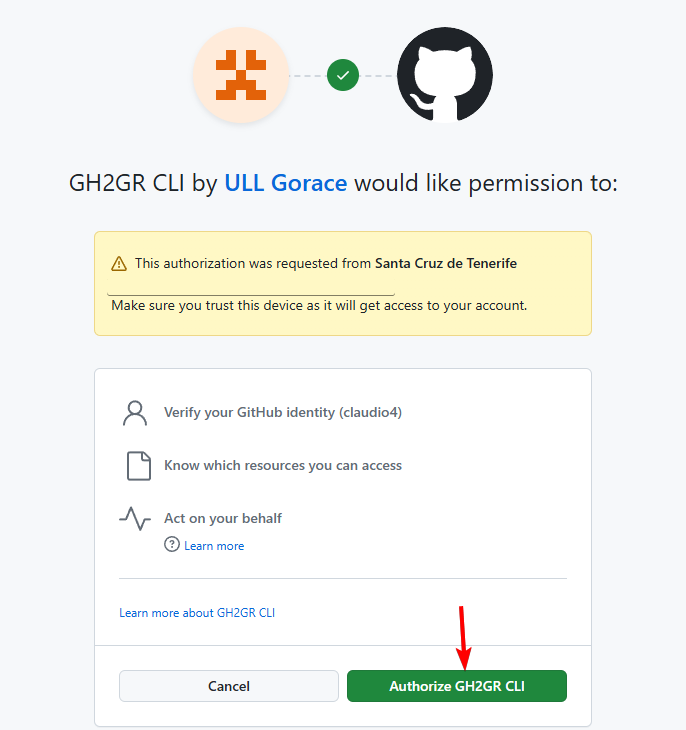
\includegraphics[width=\linewidth]{images/gh-authorize-client.png}
        \caption{Pantalla de confirmación para autorizar a GH2GR Client en la cuenta GitHub.}
        \label{fig:gh-client-login:authz}
    \end{subfigure}
    \caption{Inicio de sesión en GitHub desde GH2GR Client.}
\end{figure}

Antes de continuar, me gustaría hacer un apunte rápido para responder a la pregunta de dónde guarda el programa su configuración. La respuesta es que, si está definida la variable de entorno ``XDG\_CONFIG\_HOME'', la guardará en un subdirectorio de la ruta que la variable especifique llamado ``gh2gr''. Si la variable no está configurada, se guardará en ``~/.config'' en sistemas Linux, en ``~/Library/Application Support'' en sistemas Mac OS y en ``\%LOCALAPPDATA\%'' en sistemas Windows.

Nuestro siguiente paso será iniciar sesión en GH2GR Server. Para eso, ejecutaremos el comando \texttt{gh2gr auth gh2gr login}. Nos aparecerá un pequeño formulario (Figura \ref{fig:gh2gr-login:form}) donde nos preguntará la dirección de nuestro servidor y el token que generamos en el apartado \ref{title:add-user}. Podemos usar \textit{Tab} y \textit{Shift+Tab} para movernos abajo y arriba en el formulario, respectivamente. Cuando demos \textit{Enter} en el último campo del formulario, el programa mostrará un símbolo de carga mientras se comunica con el servidor. Si todo va correctamente, nos dirá que hemos iniciado sesión exitosamente, como en la Figura \ref{fig:gh2gr-login:ok}. 

\begin{figure}
    \begin{subfigure}{0.49\textwidth}
        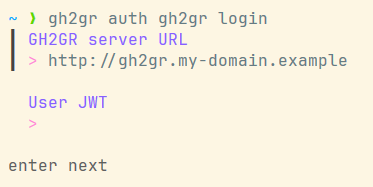
\includegraphics[width=\linewidth]{images/client-gh2gr-login-1.png}
        \caption{Formulario preguntando credenciales de GH2GR.}
        \label{fig:gh2gr-login:form}
    \end{subfigure}
    \hspace*{\fill}
    \begin{subfigure}{0.49\textwidth}
        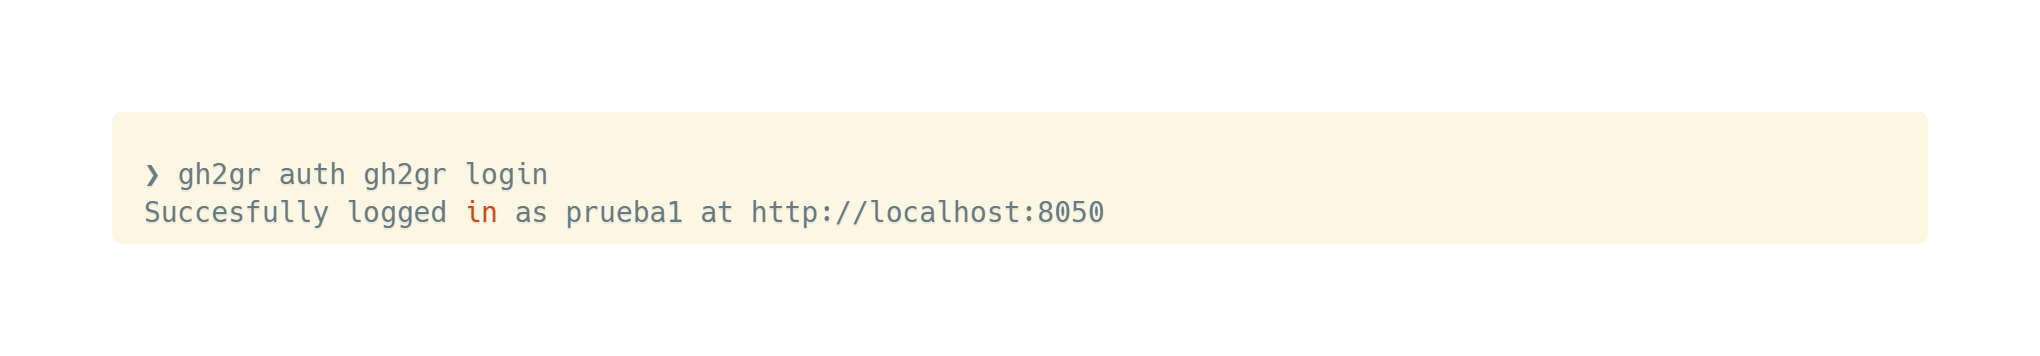
\includegraphics[width=\linewidth]{images/client-gh2gr-login-2.png}
        \caption{Ejecución exitosa del comando de iniciar sesión en GH2GR.}
        \label{fig:gh2gr-login:ok}
    \end{subfigure}
    \caption{Inicio de sesión en GH2GR.}
\end{figure}

Lo que vamos a hacer ahora no es realmente parte de la configuración del cliente, pero sí de nuestra cuenta de usuario. Vamos a enviar el token que obtuvimos al iniciar sesión en GitHub a nuestra cuenta en GH2GR Server, para permitir que este acceda a GitHub Classroom en nuestro nombre. Para ello, ejecutaremos el comando \texttt{gh2gr auth gh2gr send-github-token}. El programa nos responderá inmediatamente avisándonos de que ha enviado el token tal y como se lo hemos pedido. 

\begin{figure}[H]
    \centering
    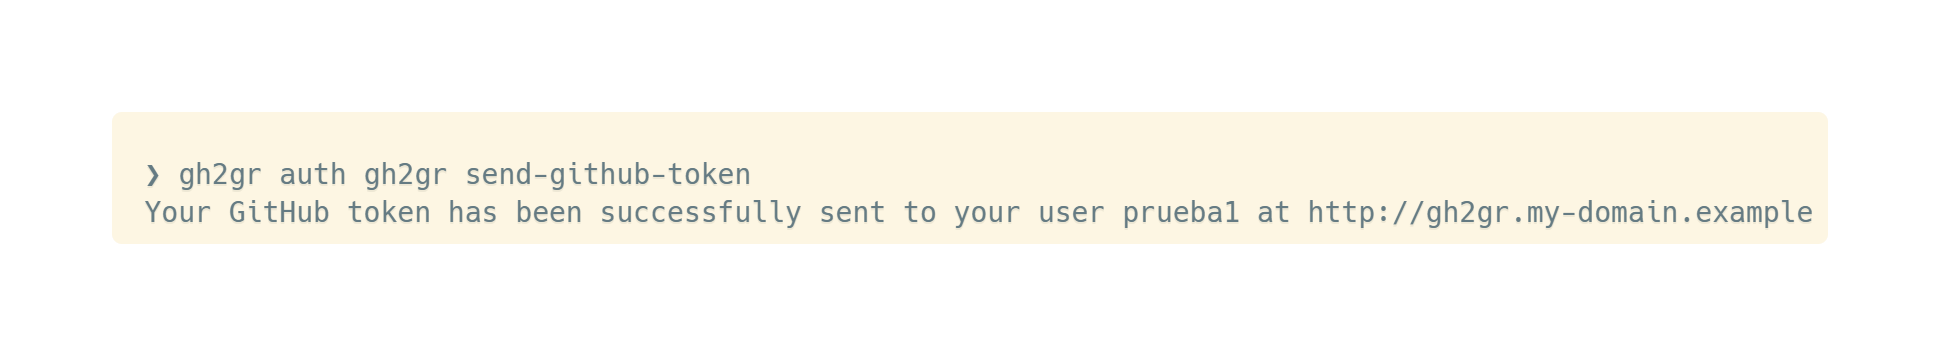
\includegraphics[width=0.75\linewidth]{images/client-gh-token-sent.png}
    \caption{Mensaje indicándonos que nuestro token de GitHub se ha enviado con éxito a nuestro usuario en GH2GR Server.}
\end{figure}

\section{Añadir una carrera}
Ahora vamos a añadir una carrera a GH2GR. Antes de poder añadir nada, necesitaremos tener una carrera ya creada en GoRace, como ya se comentó en la introducción de este capítulo.

Lo primero que tenemos que hacer es obtener el \acrshort{JWT} que nos autoriza a modificar la carrera. A continuación, se darán instrucciones de cómo proceder, pero es mejor consultar la documentación oficial de GoRace, pues, al contrario que este documento, esta puede ser actualizada si la interfaz o el procedimiento sufre algún cambio.

Primero nos dirigiremos a GoRaceAdmin y en la barra lateral pulsaremos la opción de \acrshort{API} (fig. \ref{fig:go-admin-api}). Ahora pulsaremos el botón de nuevo \acrshort{JWT} (fig. \ref{fig:go-admin-add-jwt-btn}). Tras pulsarlo, nos mostrará una confirmación (fig. \ref{fig:go-admin-add-jwt-prompt}) y, al confirmarlo, nuestro \acrshort{JWT} se habrá creado y podremos pulsar el icono de la lupa para ver su valor (fig. \ref{fig:go-admin-add-jwt-reveal}). Al pulsarla, veremos una ventana como en la figura \ref{fig:go-admin-add-jwt-value} que nos dará el valor de nuestro token. Es importante que lo tengamos a mano, pues lo necesitaremos en poco tiempo.

\begin{figure}
    \begin{subfigure}{0.18\textwidth}
        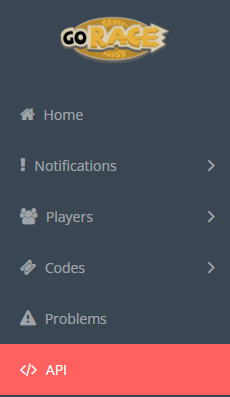
\includegraphics[width=\linewidth]{images/go-admin-api.png}
        \caption{Opción de API en la barra lateral de GoRaceAdmin.}
        \label{fig:go-admin-api}
    \end{subfigure}
    \hspace*{\fill}
    \begin{subfigure}{0.28\textwidth}
        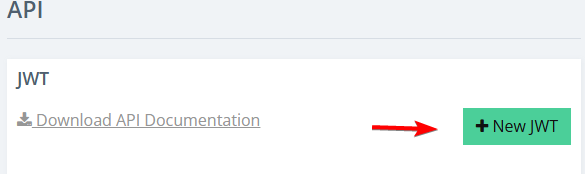
\includegraphics[width=\linewidth]{images/go-admin-add-jwt-btn.png}
        \caption{Botón para añadir un JWT en GoRaceAdmin.}
        \label{fig:go-admin-add-jwt-btn}
    \end{subfigure}
    \hspace*{\fill}
    \begin{subfigure}{0.28\textwidth}
        
\includegraphics[width=\linewidth]{images/go-admin-add-jwt-prompt.png}
        \caption{Ventana de confirmación para la creación de un nuevo JWT en GoRaceAdmin.}
        \label{fig:go-admin-add-jwt-prompt}
    \end{subfigure}
    \hspace*{\fill}
    \begin{subfigure}{0.18\textwidth}
        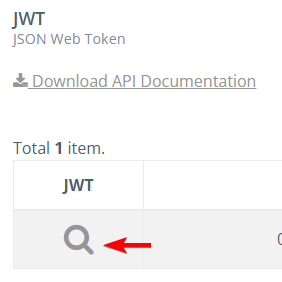
\includegraphics[width=\linewidth]{images/go-admin-add-jwt-reveal.png}
        \caption{Botón para revelar el JWT en GoRaceAdmin.}
        \label{fig:go-admin-add-jwt-reveal}
    \end{subfigure}
    \caption{Crear un JWT en GoRaceAdmin.}
\end{figure}

\begin{figure}
    \centering
    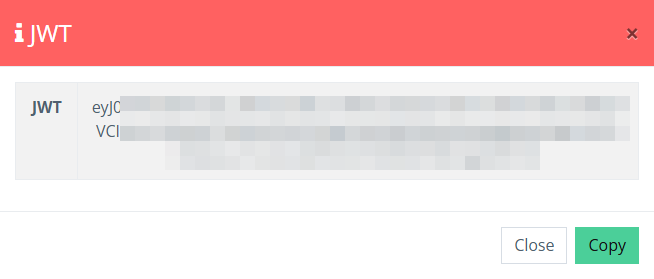
\includegraphics[width=0.5\linewidth]{go-admin-add-jwt-value.png}
    \caption{Ventana que muestra el valor del JWT en GoRaceAdmin.}
    \label{fig:go-admin-add-jwt-value}
\end{figure}

Una vez cerrado el diálogo de la figura \ref{fig:go-admin-add-jwt-value}, aprovecharemos que seguimos en el apartado de \acrshort{API} de GoRaceAdmin para añadir la \acrshort{IP} de nuestro servidor a la lista blanca de \acrshort{IP} que pueden interactuar con la \acrshort{API} de GoRace. Para ello, pulsaremos el botón verde que dice ``New IP'' (fig. \ref{fig:go-admin-add-ip-btn}). Al pulsarlo, nos aparecerá una ventana (fig. \ref{fig:go-admin-add-ip-dialog}) que nos pedirá que introduzcamos la \acrshort{IP}. Es importante resaltar que tenemos que introducir la \acrshort{IP} del servidor que ejecuta GH2GR Server, no la de ningún cliente. Una vez introducida, pulsaremos en añadir. Y listo, podemos comprobar que efectivamente nuestra \acrshort{IP} se ha añadido a la lista de \acrshort{IP} permitidas, tal y como se ve en la figura \ref{fig:go-admin-add-ip-success}.

\begin{figure}
    \begin{subfigure}{0.32\textwidth}
        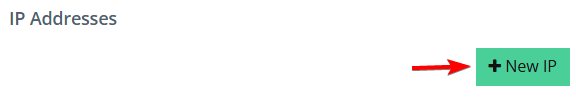
\includegraphics[width=\linewidth]{images/go-admin-add-ip-btn.png}
        \caption{Botón para añadir una IP a la lista blanca.}
        \label{fig:go-admin-add-ip-btn}
    \end{subfigure}
    \hspace*{\fill}
    \begin{subfigure}{0.32\textwidth}
        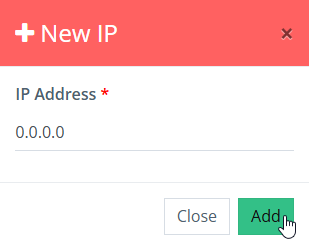
\includegraphics[width=\linewidth]{images/go-admin-add-ip-dialog.png}
        \caption{Diálogo para introducir la IP a añadir.}
        \label{fig:go-admin-add-ip-dialog}
    \end{subfigure}
    \hspace*{\fill}
    \begin{subfigure}{0.32\textwidth}
        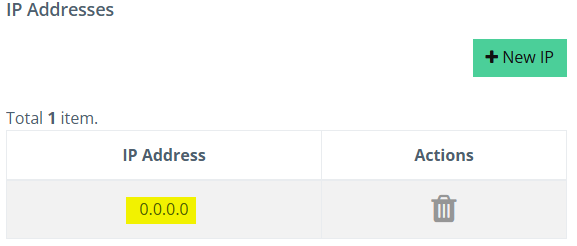
\includegraphics[width=\linewidth]{images/go-admin-add-ip-success.png}
        \caption{Lista de IP permitidas tras adición.}
        \label{fig:go-admin-add-ip-success}
    \end{subfigure}
    \caption{Permitir una IP para la API de GoRace en GoRaceAdmin.}
\end{figure}

Ahora ya podemos añadir la carrera al GH2GR. Para ello, nos dirigiremos a la terminal donde tengamos nuestro cliente y ejecutamos \texttt{gh2gr race add}. Al hacerlo, nos aparecerá un formulario (fig. \ref{fig:client-add-race-form}) para que añadamos el nombre de la carrera y el \acrshort{JWT} que acabamos de generar. Introducimos ambos datos y pulsamos \textit{Enter}. Tras unos instantes, nos dirá que nuestra carrera se ha creado con éxito.

\begin{figure}
    \centering
    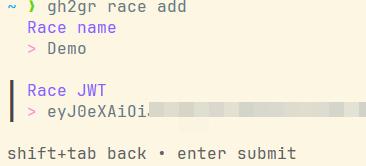
\includegraphics[width=0.5\linewidth]{images/client-add-race-form.png}
    \caption{Formulario para añadir la carrera a GH2GR.}
    \label{fig:client-add-race-form}
\end{figure}

Ahora que nuestra carrera ya está añadida, deberíamos añadir las relaciones entre los nombres de usuario de GitHub de los estudiantes y su correo electrónico. Dado que probablemente necesitemos añadir múltiples alumnos y hacerlo uno por uno puede ser tedioso, GH2GR Client acepta un \acrshort{CSV} con todos los alumnos que queramos añadir. Como es un \acrshort{CSV} común, podemos generarlo con el \textit{software} que más nos convenga, siempre que pongamos los correos electrónicos en la columna ``identifier'' y los nombres de usuario en la columna ``github\_username''. El porqué de estos nombres de columnas no es casual, y es que si usamos la función de \textit{roster} de GitHub Classroom, podremos simplemente descargarlo como se muestra en la figura \ref{fig:gh-download-roster} y utilizarlo directamente.

\begin{figure}
    \centering
    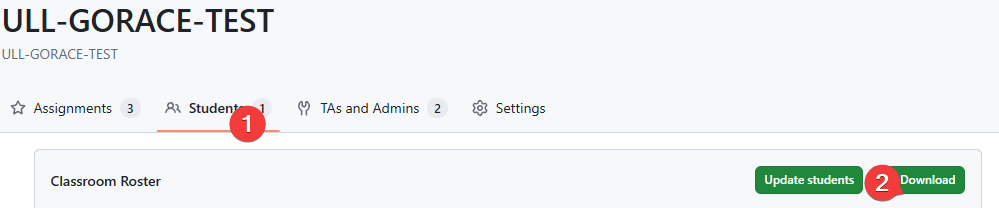
\includegraphics[width=0.5\linewidth]{images/gh-dowload-roaster.png}
    \caption{Instrucciones para descargar el \textit{roster} de GitHub Classroom.}
    \label{fig:gh-download-roster}
\end{figure}

Cuando ya tengamos nuestro \acrshort{CSV}, nos dirigiremos a la carpeta que lo albergue y ejecutaremos \texttt{gh2gr race send-roster <nombre-carrera> <fichero.csv>}. También podemos usar un guion (-) como el nombre del fichero si queremos que el programa lo lea de la entrada estándar. La terminal nos responderá que se han enviado correctamente.

\begin{figure}
    \centering
    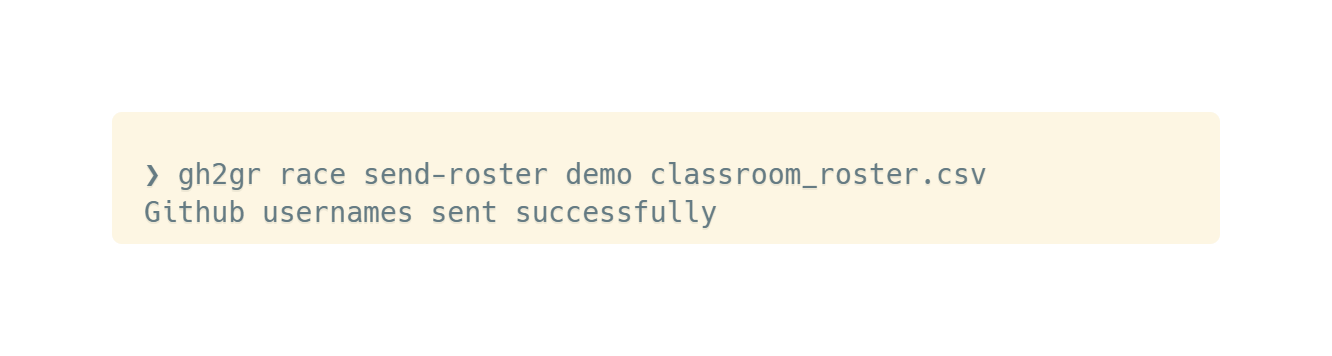
\includegraphics[width=0.5\linewidth]{images/client-send-roaster.png}
    \caption{Comando que envía la traducción entre nombre de usuario de GitHub del alumnado y sus correos electrónicos.}
\end{figure}

Un efecto secundario de enviar estas relaciones es que el servidor preregistrará a todos los correos que le hayamos otorgado en nuestra carrera en GoRace. Además, es importante comentar que podemos hacer sin ningún tipo de problema envíos parciales del \textit{roster} y estos se irán añadiendo sin problema. Además, si proporcionamos una dirección de correo electrónico distinta para un nombre que ya había sido enviado, GH2GR actualizará la traducción para usar este nuevo correo de forma silenciosa.

\section{Añadir una actividad y prepararla para su uso}

Lo último que nos resta por explicar es cómo añadir una actividad a GH2GR y prepararla para que pueda ser usada por el alumnado.

Antes de continuar, recordemos que, como siempre, se recomienda consultar la documentación oficial de GitHub además de esta guía, pues este documento corre el riesgo de quedarse desactualizado.

Lo primero que tenemos que hacer es añadir el \textit{assignment} en GitHub Classroom. Para ello, vamos a nuestro \textit{classroom} y pulsamos el botón de ``New assignment'' (fig. \ref{fig:ghc-new-assig-btn}). Al pulsarlo, nos preguntará un título (fig. \ref{fig:ghc-new-assig-1}), que podemos escoger libremente, y otras opciones que también somos libres de configurar como nos plazca. En la siguiente pantalla, es vital que escojamos un repositorio bajo nuestro control que usaremos como plantilla para el repositorio de los estudiantes (fig. \ref{fig:ghc-new-assig-2}); el resto de valores somos libres de configurarlos a nuestro gusto. En la última pantalla (fig. \ref{fig:ghc-new-assig-3}), debemos añadir las pruebas de evaluación automatizadas que consideremos, recordando que debemos agruparlas por las variables de la actividad de GoRace, usando un prefijo de ``[nombre variable]'' para este fin, tal y como se muestra en la figura \ref{fig:variable-groups-autograding-tests} y se comenta en el apartado \ref{title:mapping-gorace-gh}. También es importante añadir una puntuación a cada una de las pruebas. Tras acabar con las pruebas, podemos confirmar para crear el \textit{assignment}.

\begin{figure}
    \centering
    \begin{subfigure}{0.24\textwidth}
        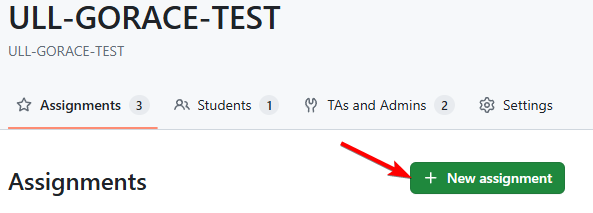
\includegraphics[width=\linewidth]{images/ghc-new-assig.btn.png}
        \caption{Botón para añadir \textit{assignment}.}
        \label{fig:ghc-new-assig-btn}
    \end{subfigure}
    \hspace*{\fill}   % maximize separation between the subfigures
    \begin{subfigure}{0.24\textwidth}
        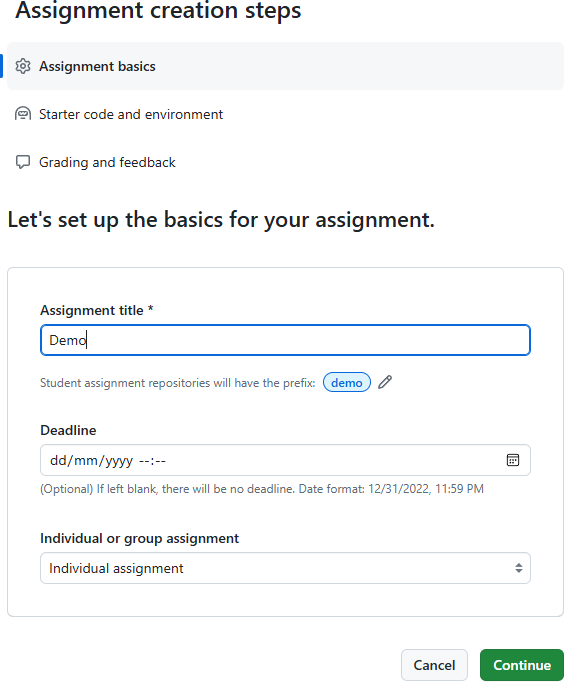
\includegraphics[width=1\linewidth]{images/ghc-new-assig-1.png}
        \caption{Pantalla inicial donde solicitan el nombre del \textit{assignment}.}
        \label{fig:ghc-new-assig-1}
    \end{subfigure}
    \hspace*{\fill}   % maximize separation between the subfigures
    \begin{subfigure}{0.24\textwidth}
        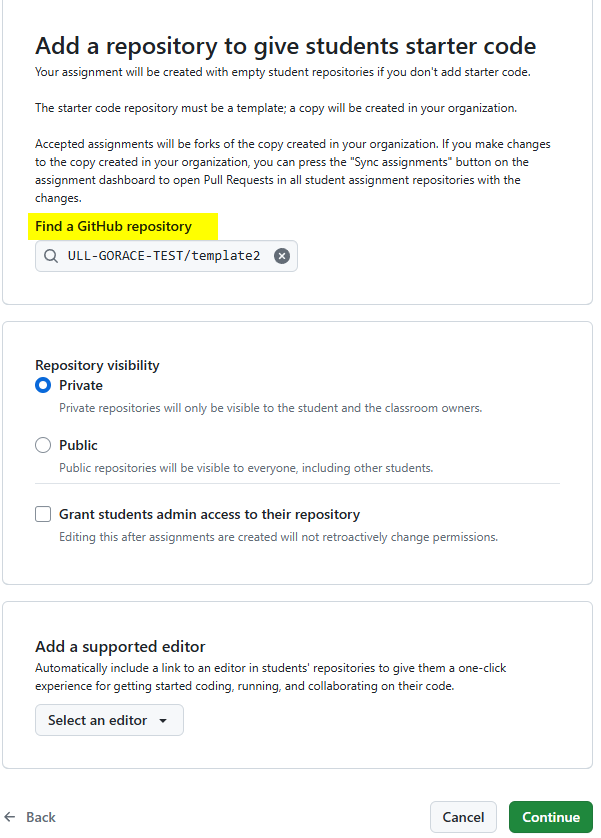
\includegraphics[width=1\linewidth]{images/ghc-new-assig-2.png}
        \caption{Pantalla donde debemos escoger el repositorio que servirá de plantilla.}
        \label{fig:ghc-new-assig-2}
    \end{subfigure}
    \hspace*{\fill}   % maximize separation between the subfigures
    \begin{subfigure}{0.24\textwidth}
       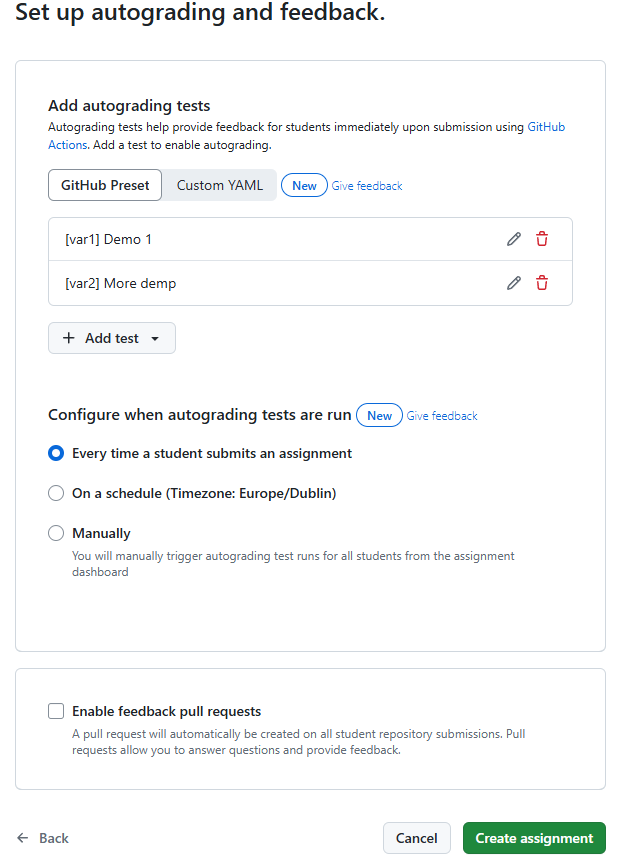
\includegraphics[width=1\linewidth]{images/ghc-new-assig-3.png}
        \caption{Pantalla donde debemos añadir las pruebas de evaluación automatizadas.}
        \label{fig:ghc-new-assig-3}
    \end{subfigure}
    \caption{Formulario para la creación de un nuevo \textit{assignment} en GitHub Classroom.}
\end{figure}

Ahora simplemente tenemos que generar el fichero de \textit{workflow} que provocará que se active la GitHub Action cuando los alumnos actualicen sus repositorios. Para ello, nos vamos a la raíz de nuestro repositorio plantilla y ejecutamos \texttt{gh2gr generate}. GH2GR nos dará una lista de las \textit{classrooms} (fig. \ref{fig:client-generate-1}) a las que nuestro usuario de GitHub tiene acceso, escogeremos la que sea adecuada. Ahora nos listará los \textit{assignments} dentro de ese \textit{classroom} (fig. \ref{fig:client-generate-2}), una vez más, escogeremos el correspondiente. A continuación, nos pedirá que escojamos una carrera de las que tenemos registradas en GH2GR (fig. \ref{fig:client-generate-3}). Tras escoger carrera, nos pedirá que escribamos el nombre de la actividad en GoRace (fig. \ref{fig:client-generate-4}) y después nos preguntará dónde debe guardar el archivo de \textit{workflow} (fig. \ref{fig:client-generate-5}). Si nos habíamos colocado en la raíz del repositorio plantilla como se indicó antes, la ruta debería ser correcta; si no, aquí tiene una oportunidad para ajustarla. Al pulsar \textit{Enter}, la aplicación generará el archivo en la ruta indicada, creando también cualquier carpeta que no existiera pero fuera parte de la ruta y nos imprimirá un mensaje de éxito (fig. \ref{fig:client-generate-6}).


\begin{figure}
    \centering
    \begin{subfigure}{0.4\textwidth}
        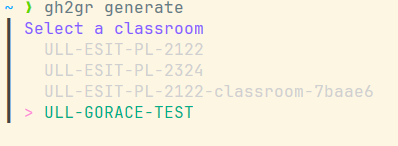
\includegraphics[width=1\linewidth]{images/client-generate-1.png}
        \caption{Menú de selección de \textit{classroom}.}
        \label{fig:client-generate-1}
    \end{subfigure}
    \hspace*{\fill}   % maximize separation between the subfigures
    \begin{subfigure}{0.4\textwidth}
        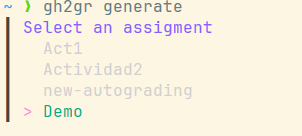
\includegraphics[width=1\linewidth]{images/client-generate-2.png}
        \caption{Menú de selección de \textit{assignment}.}
        \label{fig:client-generate-2}
    \end{subfigure}
    \\
    \begin{subfigure}{0.4\textwidth}
        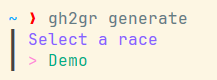
\includegraphics[width=1\linewidth]{images/client-generate-3.png}
        \caption{Menú de selección de carrera.}
        \label{fig:client-generate-3}
    \end{subfigure}
    \hspace*{\fill}   % maximize separation between the subfigures
    \begin{subfigure}{0.4\textwidth}
       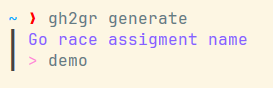
\includegraphics[width=1\linewidth]{images/client-generate-4.png}
        \caption{Entrada para el nombre de la actividad.}
        \label{fig:client-generate-4}
    \end{subfigure}
    \\
    \begin{subfigure}{0.4\textwidth}
       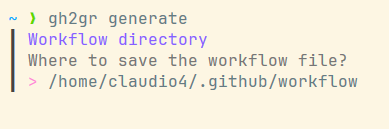
\includegraphics[width=1\linewidth]{images/client-generate-5.png}
        \caption{Entrada para el nombre de la ruta de guardado.}
        \label{fig:client-generate-5}
    \end{subfigure}
    \hspace*{\fill}
    \begin{subfigure}{0.4\textwidth}
       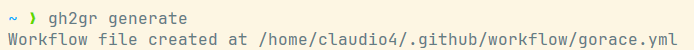
\includegraphics[width=1\linewidth]{images/client-generate-6.png}
        \caption{Salida confirmando el guardado del fichero.}
        \label{fig:client-generate-6}
    \end{subfigure}
    \caption{Comando de gh2gr generate.}
\end{figure}

Con esto, solo tendremos que hacer \textit{commit} y \textit{push}, y ya estará todo listo para que nuestros alumnos puedan disfrutar de la integración entre GitHub Classroom y GoRace.
